\documentclass[landscape]{article}

\usepackage[utf8]{inputenc}
\usepackage[english]{babel}

\usepackage{amsmath,amsfonts,amssymb}
\usepackage{fullpage}
\usepackage{verbatim}

\usepackage[margin=10mm, top=10mm, bottom=5mm]{geometry}

\usepackage{tikz,pgfplots}

\pgfplotsset{
  width=240mm,height=190mm,
  major grid style={thin,dotted,color=black!50},
  minor grid style={thin,dotted,color=black!50},
  grid,
  every axis/.append style={
    line width=0.5pt,
    tick style={
      line cap=round,
      thin,
      major tick length=4pt,
      minor tick length=2pt,
    },
  },
  legend cell align=left,
  legend pos=north east,
  compat=1.9
}

%%%%%%%%%%%%%%%%%%%%%%%%%%%%%%%%%%%%%%%%%%%%%%%%%%%%%%%%%%%%%%%%%%%%%%%%%%%%%%%%

\begin{document}

% IMPORT-DATA ResultsQS schizo_hcq_juqueen.txt

%%%%%%%%%%%%%%%%%%%%%%%%%%%%%%%%%%%%%%%%%%%%%%%%%%%%%%%%%%%%%%%%%%%%%%%%%%%%%%%%

\begin{center}


\begin{tikzpicture}
  \begin{axis}[
    title={8k cores, uniform input},
    xlabel={Elements [$\log_2(n)$]},
    ylabel={Run Time},
    xmajorgrids=false,
    xtick={0,...,20},
    ytick={0,2e-3,4e-3,6e-3,8e-3,1e-2,1.2e-2,1.4e-2,1.6e-2,1.8e-2,2e-2},
    ymin=0,   
    ymax=2e-2,
    legend pos=north west,
    ]   
	%% MULTIPLOT(algo) SELECT  LOG(2,`n-p`) AS x, MEDIAN(`wall-time`) as y, MULTIPLOT
	%% FROM ResultsQS
	%% WHERE p=8192  AND generator="UniformGeneratorMechanism" AND x<=10
	%% GROUP BY MULTIPLOT, x  ORDER BY MULTIPLOT, x
 \addplot coordinates { (0.0,0.003483) (1.0,0.003408) (2.0,0.003403) (3.0,0.003429) (4.0,0.003525) (5.0,0.0037355) (6.0,0.0038985) (7.0,0.004089) (8.0,0.004256) (9.0,0.0045305) (10.0,0.0049935) };
 \addlegendentry{algo=LightSplitParQsortDistTwoDistSorterMechanism<LightSplitBinTreeKMedianSelect,KNeighborhoodPivotSelectorMechanism>};
 \addplot coordinates { (0.0,0.0135025) (1.0,0.014207) (2.0,0.014853) (3.0,0.015009) (4.0,0.0152155) (5.0,0.0153485) (6.0,0.015663) (7.0,0.015843) (8.0,0.0159975) (9.0,0.016514) (10.0,0.016559) };
 \addlegendentry{algo=SchizoQSDistTwoDistSorterMechanism};

  \end{axis}
\end{tikzpicture}
\newpage

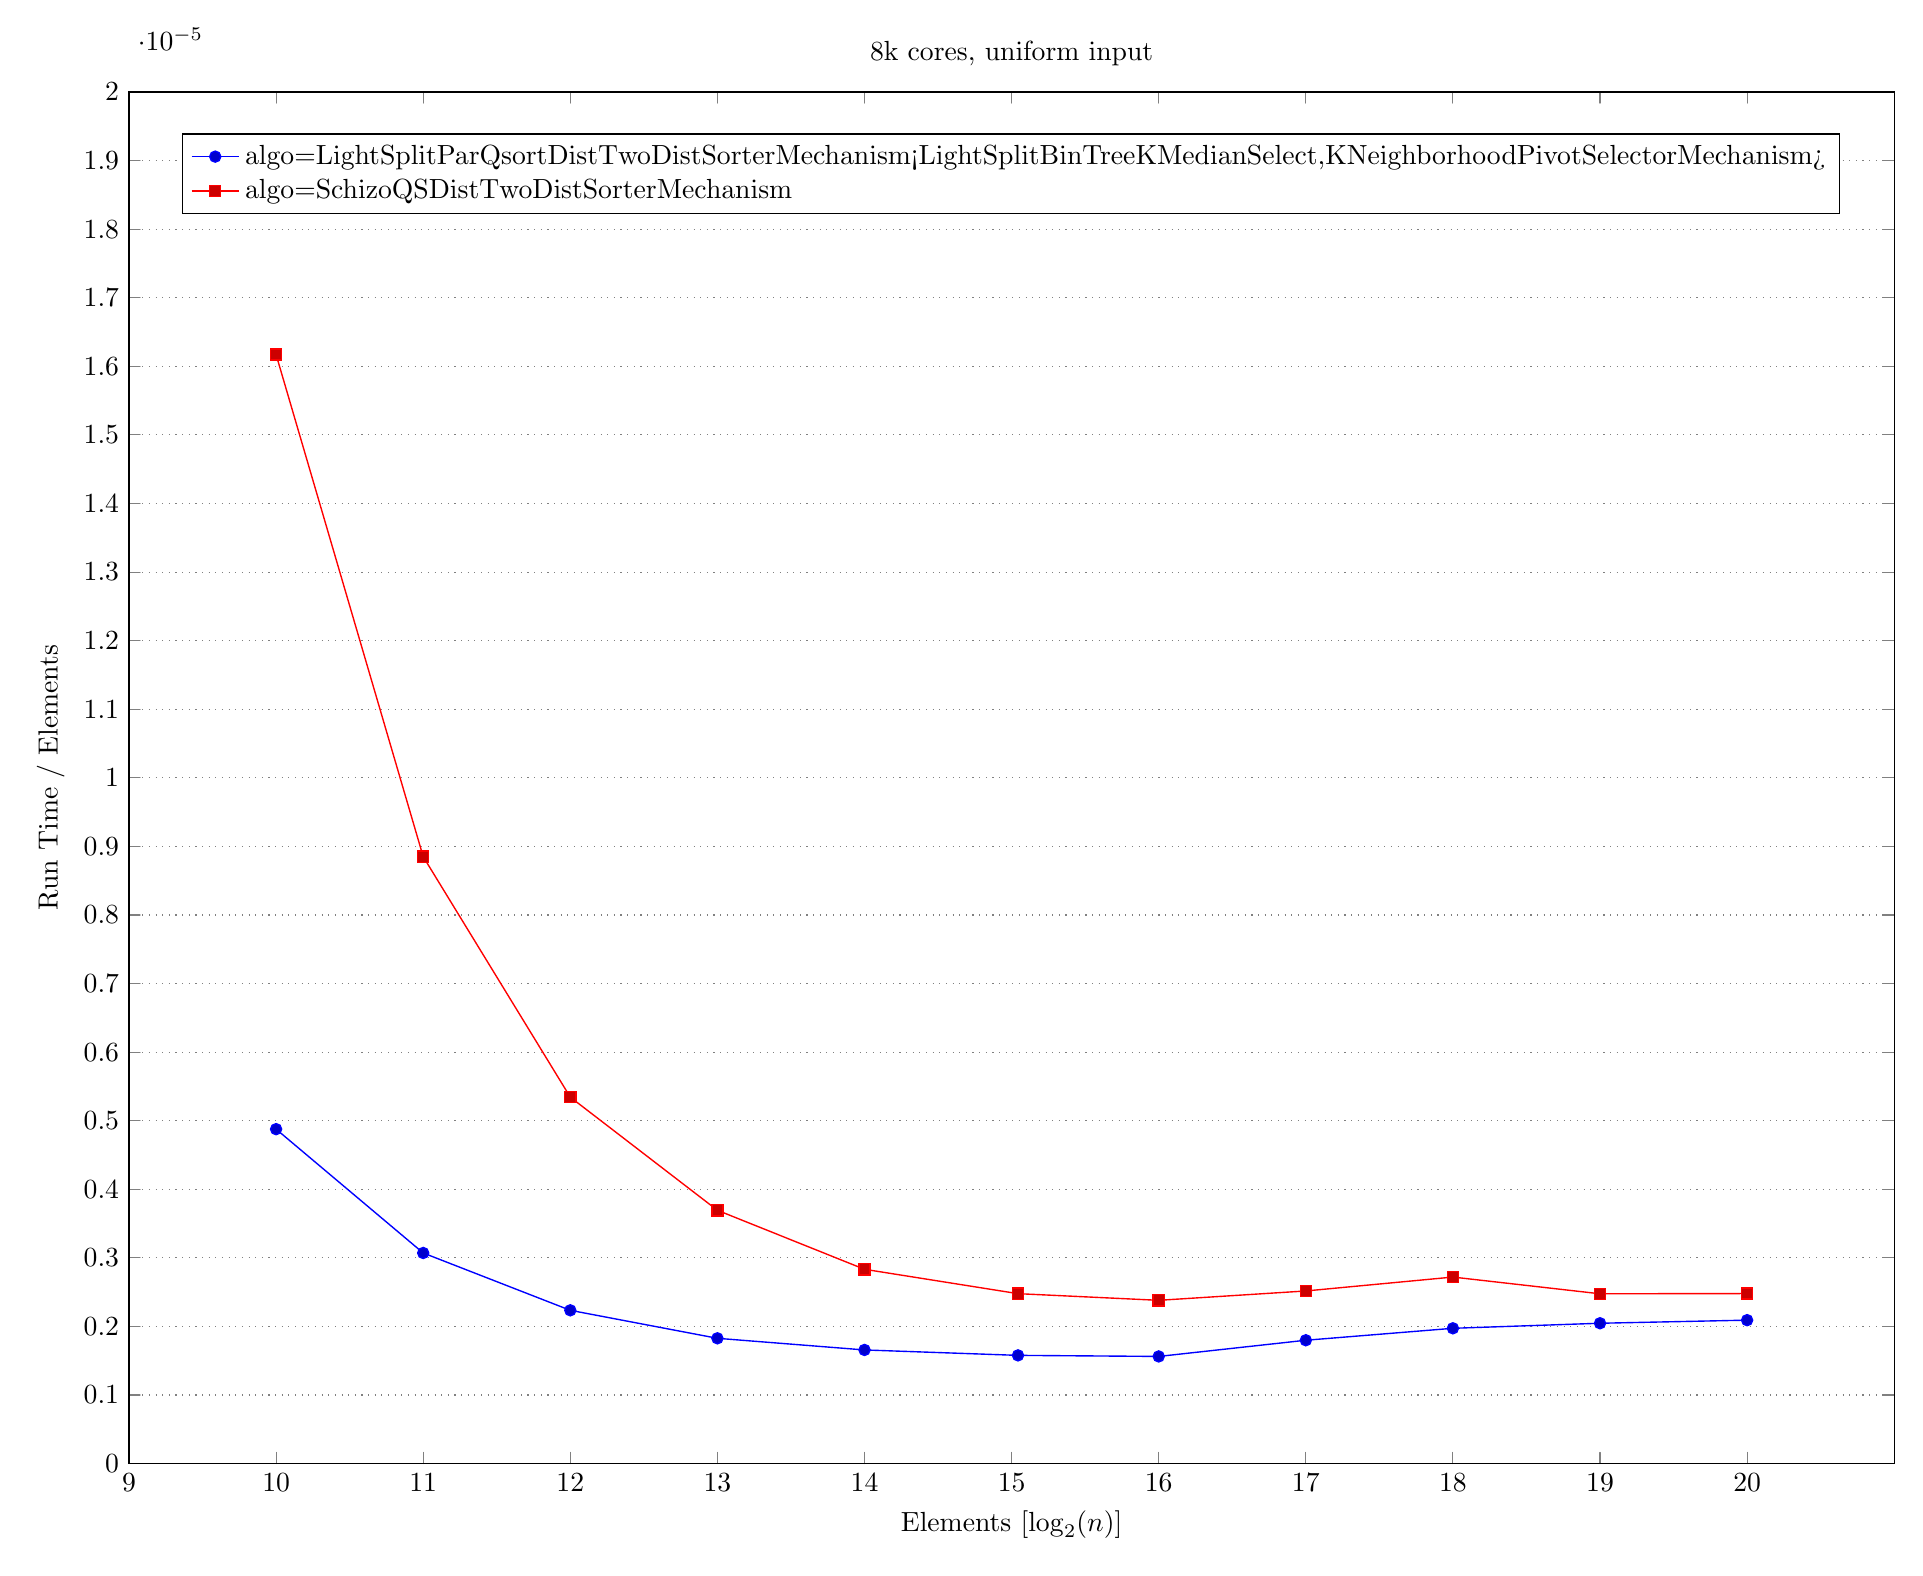
\begin{tikzpicture}
  \begin{axis}[
    title={8k cores, uniform input},
    xlabel={Elements [$\log_2(n)$]},
    ylabel={Run Time / Elements},
    xmajorgrids=false,
    xtick={0,...,20},
    ymin=0, 
    ymax=2e-5,  
    legend pos=north west,
    ]   
	%% MULTIPLOT(algo) SELECT  LOG(2,`n-p`) AS x, MEDIAN(`wall-time`)/`n-p` as y, MULTIPLOT
	%% FROM ResultsQS
	%% WHERE p=8192  AND generator="UniformGeneratorMechanism" AND x>=10
	%% GROUP BY MULTIPLOT, x  ORDER BY MULTIPLOT, x
 \addplot coordinates { (10.0,4.87646e-06) (11.0,3.0708e-06) (12.0,2.23474e-06) (13.0,1.82654e-06) (14.0,1.6568e-06) (15.0434,1.57771e-06) (16.0,1.56219e-06) (17.0,1.79824e-06) (18.0,1.97251e-06) (19.0,2.04606e-06) (20.0,2.09116e-06) };
 \addlegendentry{algo=LightSplitParQsortDistTwoDistSorterMechanism<LightSplitBinTreeKMedianSelect,KNeighborhoodPivotSelectorMechanism>};
 \addplot coordinates { (10.0,1.61709e-05) (11.0,8.84961e-06) (12.0,5.34277e-06) (13.0,3.69324e-06) (14.0,2.83298e-06) (15.0434,2.47758e-06) (16.0,2.38049e-06) (17.0,2.51684e-06) (18.0,2.71963e-06) (19.0,2.47575e-06) (20.0,2.47925e-06) };
 \addlegendentry{algo=SchizoQSDistTwoDistSorterMechanism};

  \end{axis}
\end{tikzpicture}
\newpage

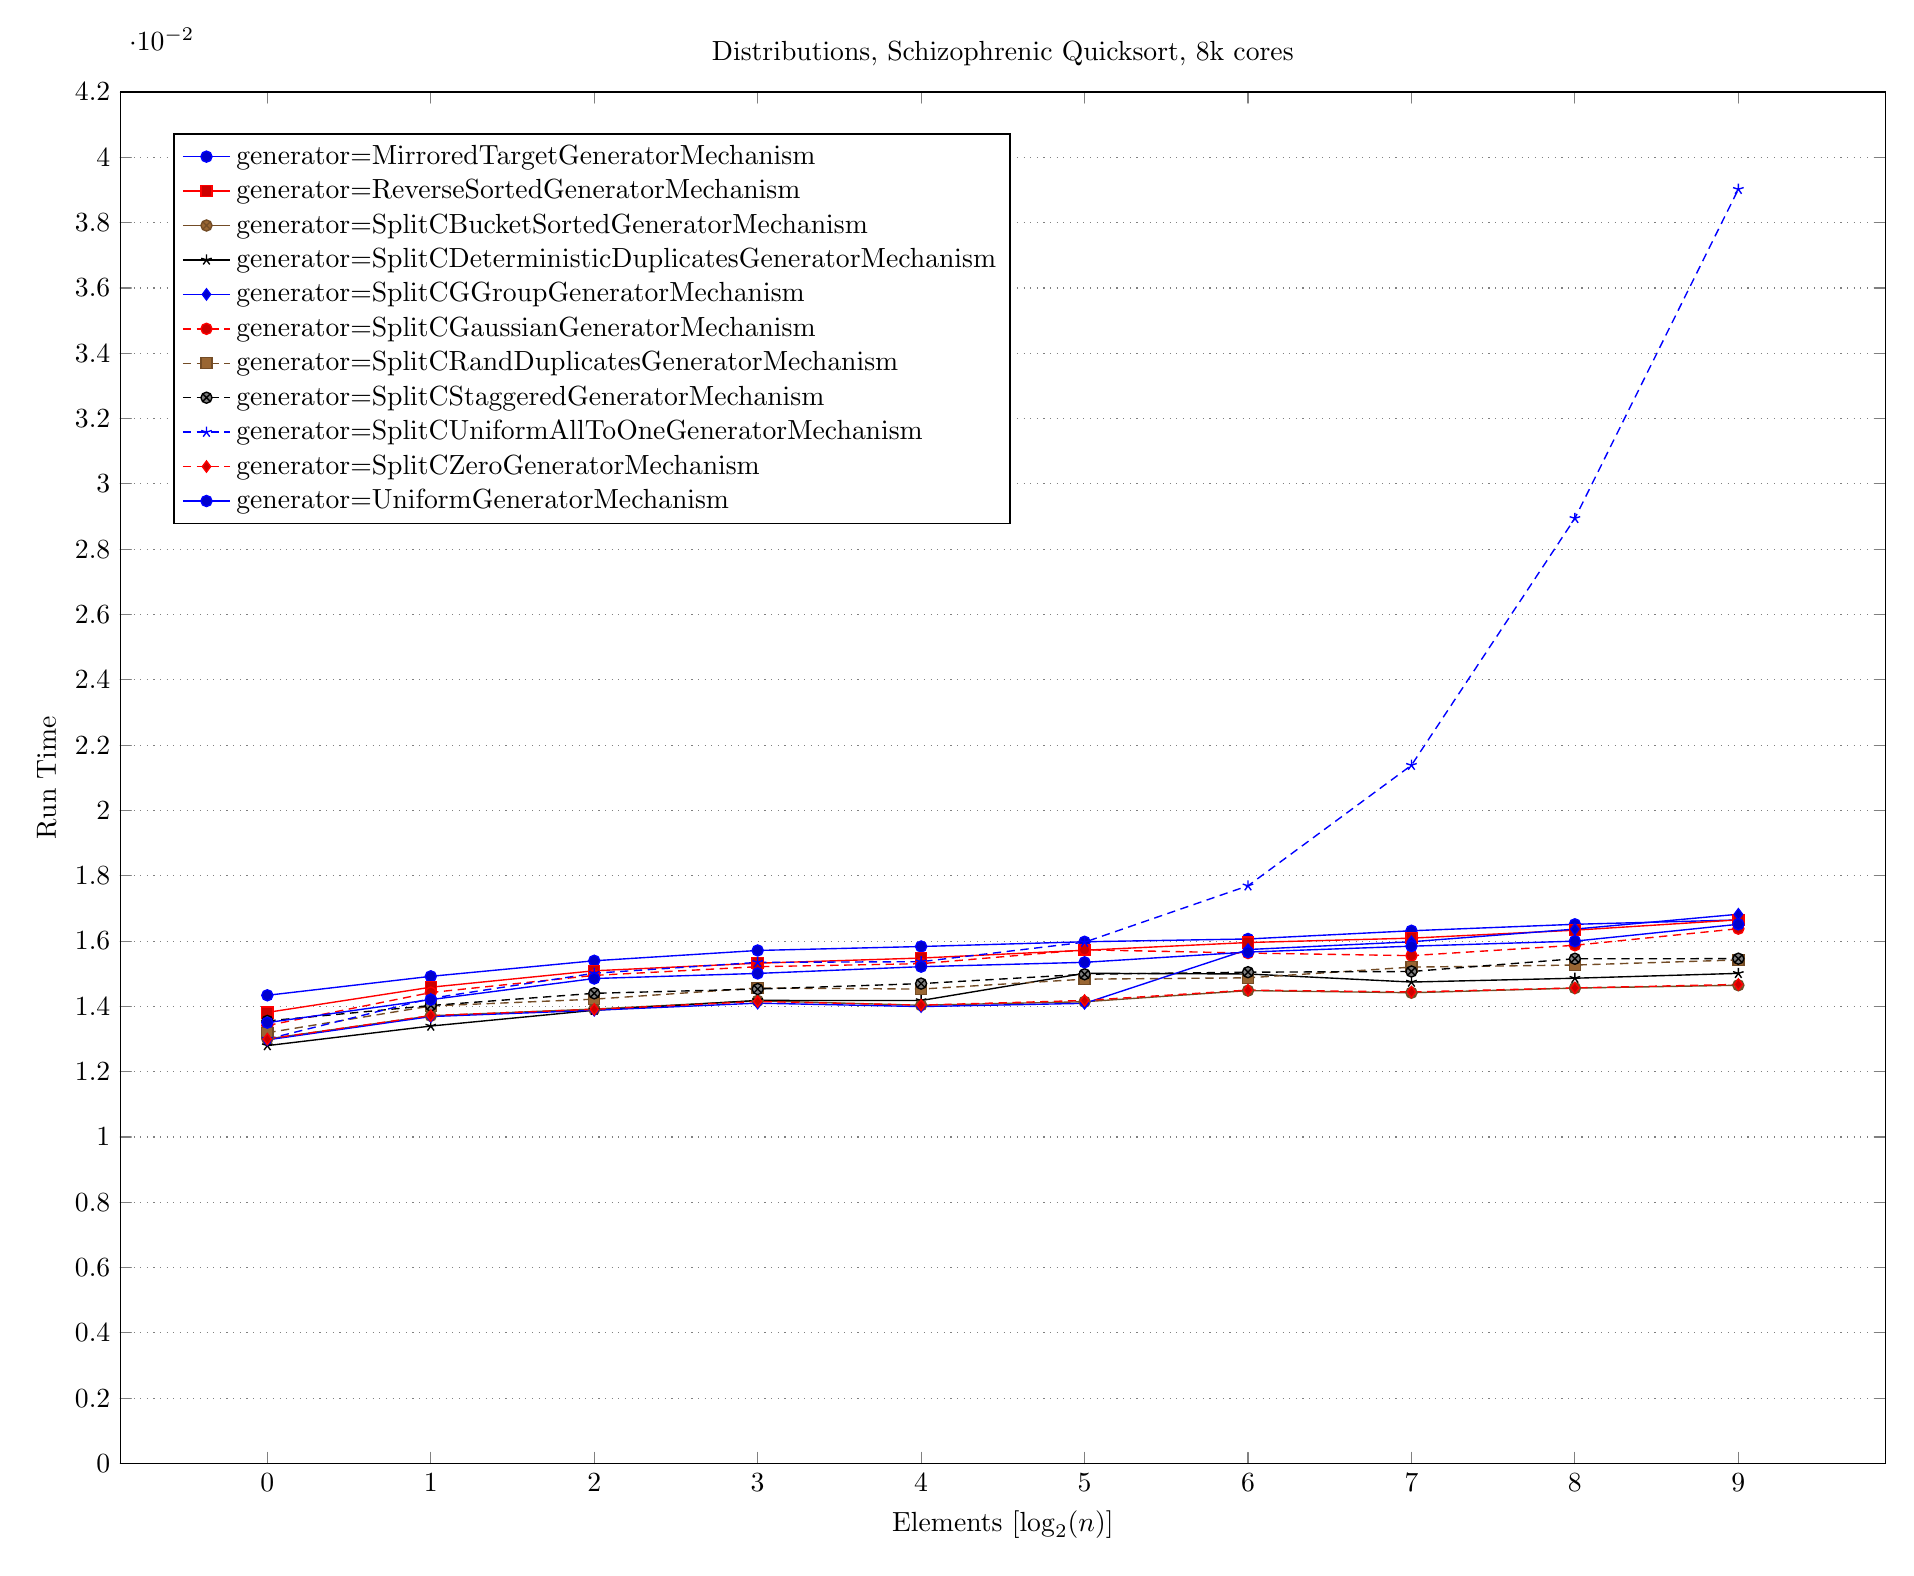
\begin{tikzpicture}
  \begin{axis}[
    title={Distributions, Schizophrenic Quicksort, 8k cores},
    xlabel={Elements [$\log_2(n)$]},
    xmajorgrids=false,
    xtick={0,...,20},
    ylabel={Run Time},
    ymin=0,   
    ymax=4.2e-2,
    legend pos=north west,
    ]   
	%% MULTIPLOT(generator) SELECT  LOG(2,`n-p`) AS x, MEDIAN(`wall-time`) as y, MULTIPLOT
	%% FROM ResultsQS
	%% WHERE p=8192  AND algo="SchizoQSDistTwoDistSorterMechanism" AND x<10
	%% GROUP BY MULTIPLOT, x  ORDER BY MULTIPLOT, x
 \addplot coordinates { (0.0,0.014339) (1.0,0.01492) (2.0,0.0153965) (3.0,0.015712) (4.0,0.015833) (5.0,0.0159785) (6.0,0.016064) (7.0,0.0163155) (8.0,0.0165135) (9.0,0.016647) };
 \addlegendentry{generator=MirroredTargetGeneratorMechanism};
 \addplot coordinates { (0.0,0.013815) (1.0,0.0145865) (2.0,0.01509) (3.0,0.0153215) (4.0,0.01548) (5.0,0.0157185) (6.0,0.0159555) (7.0,0.016089) (8.0,0.016333) (9.0,0.01665) };
 \addlegendentry{generator=ReverseSortedGeneratorMechanism};
 \addplot coordinates { (0.0,0.0130015) (1.0,0.0137115) (2.0,0.0139175) (3.0,0.014171) (4.0,0.014034) (5.0,0.0141415) (6.0,0.0144825) (7.0,0.0144175) (8.0,0.0145595) (9.0,0.0146465) };
 \addlegendentry{generator=SplitCBucketSortedGeneratorMechanism};
 \addplot coordinates { (0.0,0.0127985) (1.0,0.0133975) (2.0,0.0138805) (3.0,0.014182) (4.0,0.01418) (5.0,0.015013) (6.0,0.014992) (7.0,0.0147445) (8.0,0.014862) (9.0,0.0150105) };
 \addlegendentry{generator=SplitCDeterministicDuplicatesGeneratorMechanism};
 \addplot coordinates { (0.0,0.0129745) (1.0,0.0136875) (2.0,0.0138805) (3.0,0.0140985) (4.0,0.013994) (5.0,0.0140925) (6.0,0.0157405) (7.0,0.0159785) (8.0,0.016366) (9.0,0.0168215) };
 \addlegendentry{generator=SplitCGGroupGeneratorMechanism};
 \addplot coordinates { (0.0,0.013413) (1.0,0.0144235) (2.0,0.0149485) (3.0,0.015215) (4.0,0.0153075) (5.0,0.015733) (6.0,0.0156325) (7.0,0.0155535) (8.0,0.0158705) (9.0,0.016379) };
 \addlegendentry{generator=SplitCGaussianGeneratorMechanism};
 \addplot coordinates { (0.0,0.0131925) (1.0,0.0140115) (2.0,0.0142205) (3.0,0.014563) (4.0,0.0145295) (5.0,0.0148335) (6.0,0.014874) (7.0,0.0152015) (8.0,0.0152655) (9.0,0.015422) };
 \addlegendentry{generator=SplitCRandDuplicatesGeneratorMechanism};
 \addplot coordinates { (0.0,0.0135535) (1.0,0.0140265) (2.0,0.0144) (3.0,0.01453) (4.0,0.014697) (5.0,0.0149835) (6.0,0.015047) (7.0,0.015068) (8.0,0.015459) (9.0,0.0154605) };
 \addlegendentry{generator=SplitCStaggeredGeneratorMechanism};
 \addplot coordinates { (0.0,0.012999) (1.0,0.0142455) (2.0,0.015015) (3.0,0.0153475) (4.0,0.015368) (5.0,0.015965) (6.0,0.017692) (7.0,0.021384) (8.0,0.0289445) (9.0,0.0390215) };
 \addlegendentry{generator=SplitCUniformAllToOneGeneratorMechanism};
 \addplot coordinates { (0.0,0.0130005) (1.0,0.013719) (2.0,0.01391) (3.0,0.0141505) (4.0,0.0140385) (5.0,0.0141805) (6.0,0.0144995) (7.0,0.0144415) (8.0,0.014565) (9.0,0.014673) };
 \addlegendentry{generator=SplitCZeroGeneratorMechanism};
 \addplot coordinates { (0.0,0.0135025) (1.0,0.014207) (2.0,0.014853) (3.0,0.015009) (4.0,0.0152155) (5.0,0.0153485) (6.0,0.015663) (7.0,0.015843) (8.0,0.0159975) (9.0,0.016514) };
 \addlegendentry{generator=UniformGeneratorMechanism};

  \end{axis}
\end{tikzpicture}
\newpage

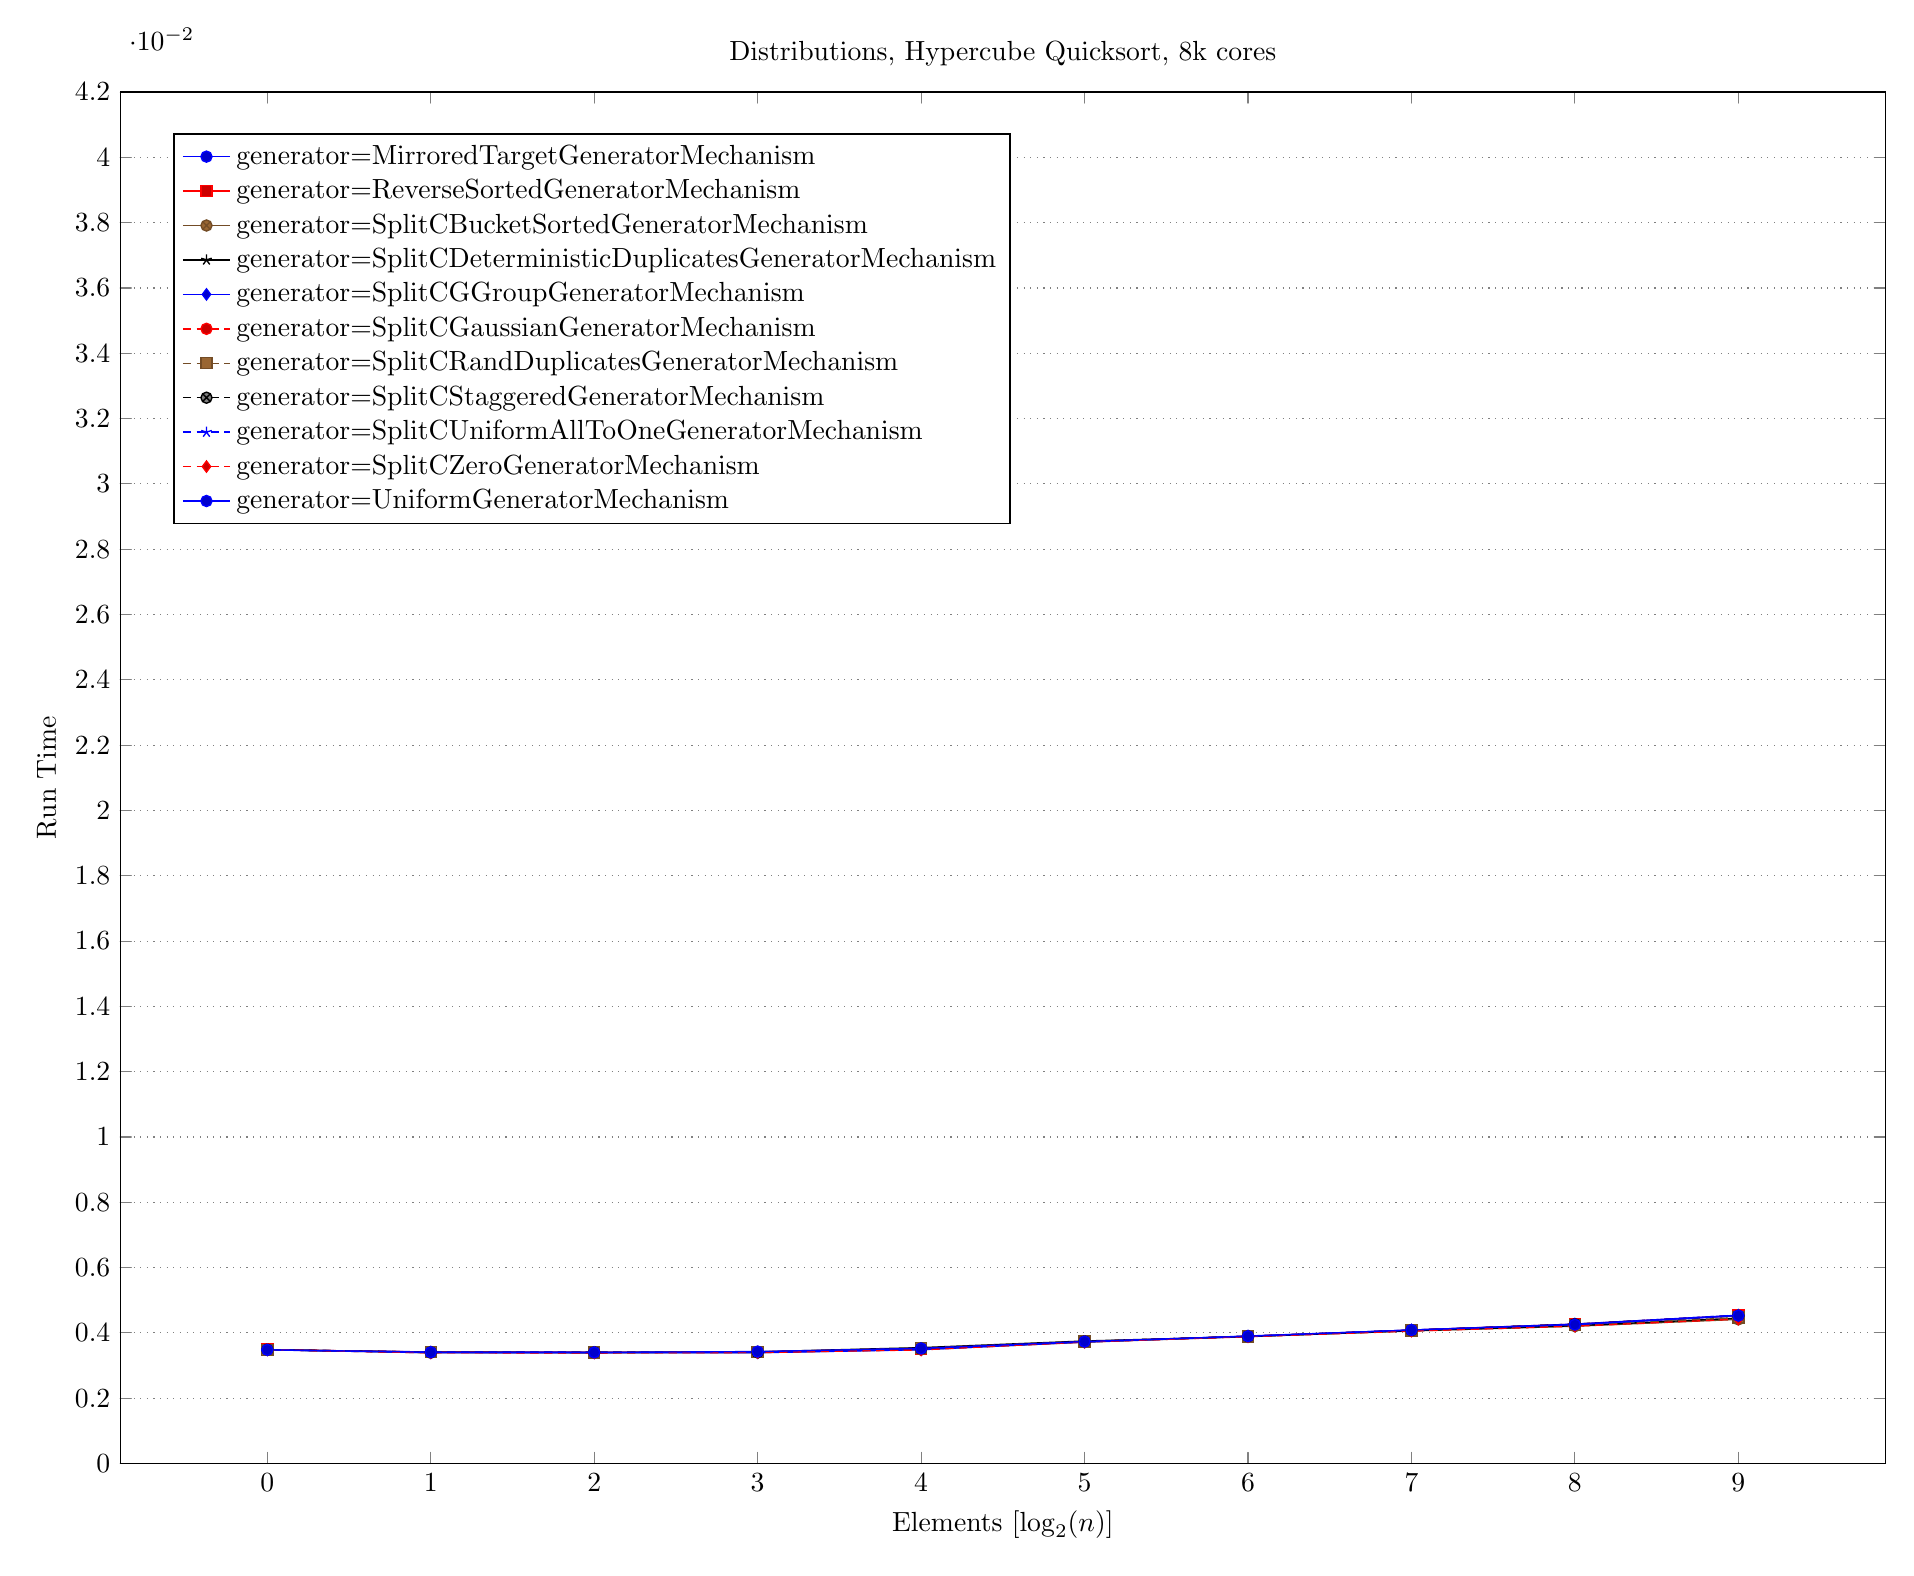
\begin{tikzpicture}
  \begin{axis}[
    title={Distributions, Hypercube Quicksort, 8k cores},
    xlabel={Elements [$\log_2(n)$]},
    ylabel={Run Time},
    xmajorgrids=false,
    xtick={0,...,20},
    ymin=0,
    ymax=4.2e-2,
    legend pos=north west,
    ]   
	%% MULTIPLOT(generator) SELECT  LOG(2,`n-p`) AS x, MEDIAN(`wall-time`) as y, MULTIPLOT
	%% FROM ResultsQS
	%% WHERE p=8192  AND algo="LightSplitParQsortDistTwoDistSorterMechanism<LightSplitBinTreeKMedianSelect,KNeighborhoodPivotSelectorMechanism>" AND x<10
	%% GROUP BY MULTIPLOT, x  ORDER BY MULTIPLOT, x
 \addplot coordinates { (0.0,0.003483) (1.0,0.003417) (2.0,0.0034095) (3.0,0.003407) (4.0,0.003525) (5.0,0.003725) (6.0,0.0038905) (7.0,0.0040865) (8.0,0.004258) (9.0,0.004528) };
 \addlegendentry{generator=MirroredTargetGeneratorMechanism};
 \addplot coordinates { (0.0,0.003487) (1.0,0.003413) (2.0,0.003405) (3.0,0.0034175) (4.0,0.003529) (5.0,0.00373) (6.0,0.003893) (7.0,0.004085) (8.0,0.0042675) (9.0,0.004533) };
 \addlegendentry{generator=ReverseSortedGeneratorMechanism};
 \addplot coordinates { (0.0,0.0034895) (1.0,0.003391) (2.0,0.0033955) (3.0,0.0033985) (4.0,0.00349) (5.0,0.0037165) (6.0,0.003891) (7.0,0.004061) (8.0,0.004206) (9.0,0.004415) };
 \addlegendentry{generator=SplitCBucketSortedGeneratorMechanism};
 \addplot coordinates { (0.0,0.003484) (1.0,0.0034095) (2.0,0.003397) (3.0,0.0034215) (4.0,0.00355) (5.0,0.0037525) (6.0,0.003889) (7.0,0.004068) (8.0,0.0042205) (9.0,0.0044535) };
 \addlegendentry{generator=SplitCDeterministicDuplicatesGeneratorMechanism};
 \addplot coordinates { (0.0,0.0034815) (1.0,0.003395) (2.0,0.003391) (3.0,0.0033945) (4.0,0.003486) (5.0,0.003723) (6.0,0.003905) (7.0,0.0040875) (8.0,0.0042705) (9.0,0.004542) };
 \addlegendentry{generator=SplitCGGroupGeneratorMechanism};
 \addplot coordinates { (0.0,0.0034885) (1.0,0.0034105) (2.0,0.0034025) (3.0,0.003418) (4.0,0.003522) (5.0,0.0037315) (6.0,0.0039) (7.0,0.0040815) (8.0,0.004263) (9.0,0.004533) };
 \addlegendentry{generator=SplitCGaussianGeneratorMechanism};
 \addplot coordinates { (0.0,0.003482) (1.0,0.0034105) (2.0,0.003404) (3.0,0.003409) (4.0,0.003534) (5.0,0.003741) (6.0,0.0038915) (7.0,0.00407) (8.0,0.004237) (9.0,0.0044685) };
 \addlegendentry{generator=SplitCRandDuplicatesGeneratorMechanism};
 \addplot coordinates { (0.0,0.0034865) (1.0,0.0034085) (2.0,0.0034055) (3.0,0.0034095) (4.0,0.0035185) (5.0,0.003737) (6.0,0.0038965) (7.0,0.0040825) (8.0,0.004269) (9.0,0.004527) };
 \addlegendentry{generator=SplitCStaggeredGeneratorMechanism};
 \addplot coordinates { (0.0,0.0034815) (1.0,0.003415) (2.0,0.003409) (3.0,0.003409) (4.0,0.003527) (5.0,0.003728) (6.0,0.003896) (7.0,0.0040805) (8.0,0.0042625) (9.0,0.0045465) };
 \addlegendentry{generator=SplitCUniformAllToOneGeneratorMechanism};
 \addplot coordinates { (0.0,0.0034865) (1.0,0.003392) (2.0,0.00339) (3.0,0.0034) (4.0,0.0034805) (5.0,0.0037225) (6.0,0.0038835) (7.0,0.0040565) (8.0,0.004207) (9.0,0.0044215) };
 \addlegendentry{generator=SplitCZeroGeneratorMechanism};
 \addplot coordinates { (0.0,0.003483) (1.0,0.003408) (2.0,0.003403) (3.0,0.003429) (4.0,0.003525) (5.0,0.0037355) (6.0,0.0038985) (7.0,0.004089) (8.0,0.004256) (9.0,0.0045305) };
 \addlegendentry{generator=UniformGeneratorMechanism};

  \end{axis}
\end{tikzpicture}
\newpage

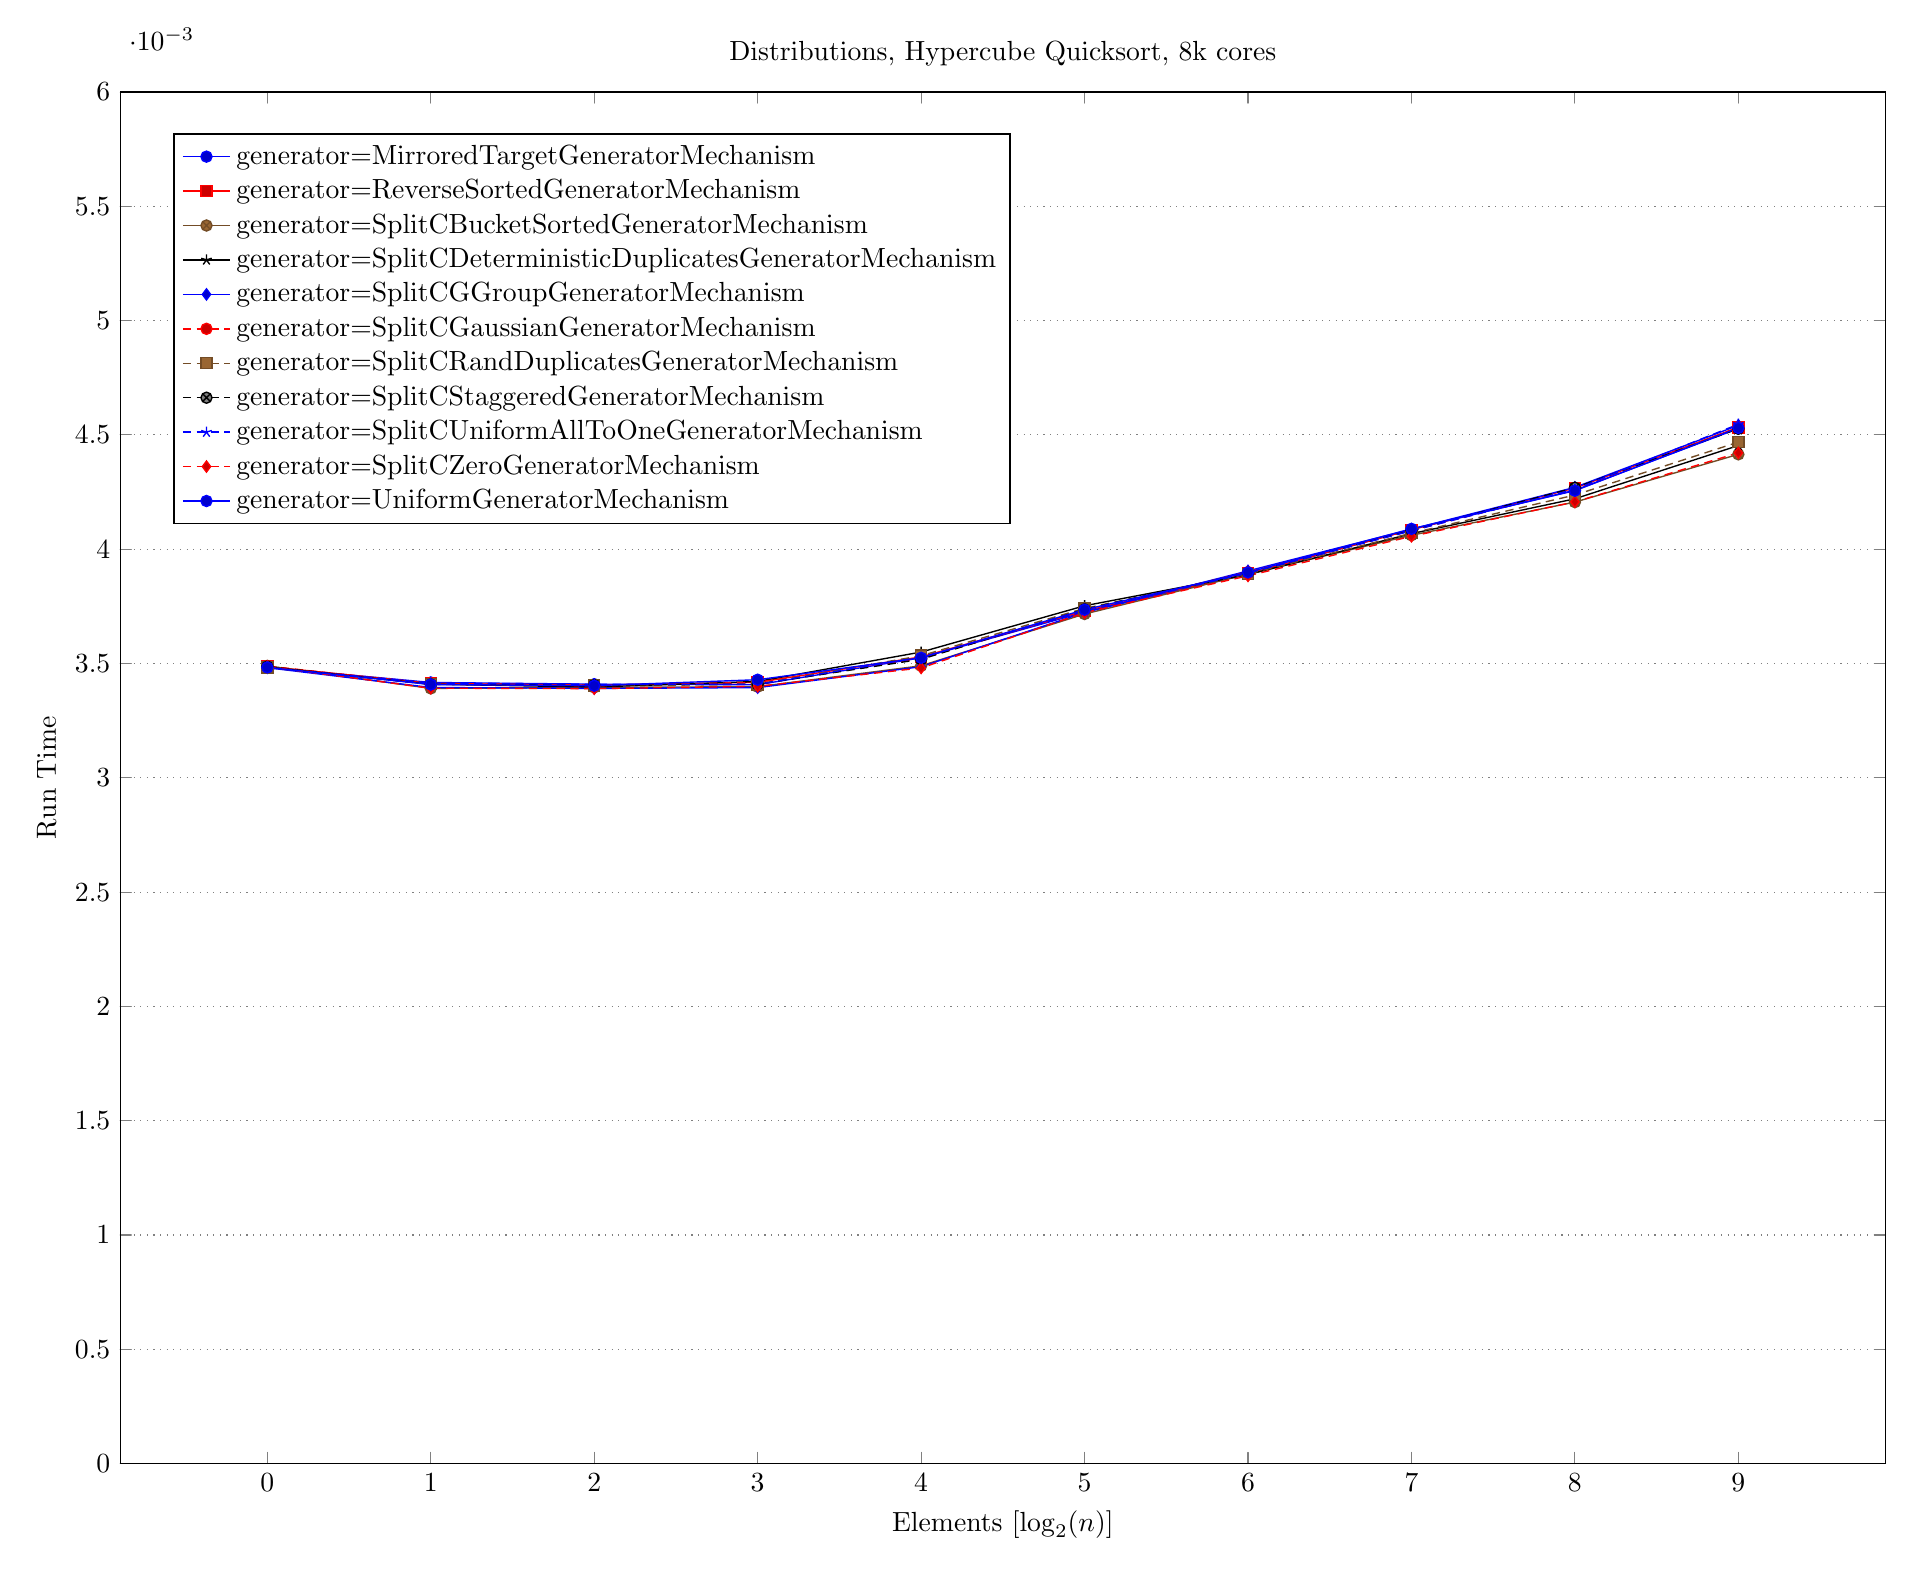
\begin{tikzpicture}
  \begin{axis}[
    title={Distributions, Hypercube Quicksort, 8k cores},
    xlabel={Elements [$\log_2(n)$]},
    ylabel={Run Time},
    xmajorgrids=false,
    xtick={0,...,20},
    ymin=0,
    ymax=6e-3,
    legend pos=north west,
    ]   
	%% MULTIPLOT(generator) SELECT  LOG(2,`n-p`) AS x, MEDIAN(`wall-time`) as y, MULTIPLOT
	%% FROM ResultsQS
	%% WHERE p=8192  AND algo="LightSplitParQsortDistTwoDistSorterMechanism<LightSplitBinTreeKMedianSelect,KNeighborhoodPivotSelectorMechanism>" AND x<10
	%% GROUP BY MULTIPLOT, x  ORDER BY MULTIPLOT, x
 \addplot coordinates { (0.0,0.003483) (1.0,0.003417) (2.0,0.0034095) (3.0,0.003407) (4.0,0.003525) (5.0,0.003725) (6.0,0.0038905) (7.0,0.0040865) (8.0,0.004258) (9.0,0.004528) };
 \addlegendentry{generator=MirroredTargetGeneratorMechanism};
 \addplot coordinates { (0.0,0.003487) (1.0,0.003413) (2.0,0.003405) (3.0,0.0034175) (4.0,0.003529) (5.0,0.00373) (6.0,0.003893) (7.0,0.004085) (8.0,0.0042675) (9.0,0.004533) };
 \addlegendentry{generator=ReverseSortedGeneratorMechanism};
 \addplot coordinates { (0.0,0.0034895) (1.0,0.003391) (2.0,0.0033955) (3.0,0.0033985) (4.0,0.00349) (5.0,0.0037165) (6.0,0.003891) (7.0,0.004061) (8.0,0.004206) (9.0,0.004415) };
 \addlegendentry{generator=SplitCBucketSortedGeneratorMechanism};
 \addplot coordinates { (0.0,0.003484) (1.0,0.0034095) (2.0,0.003397) (3.0,0.0034215) (4.0,0.00355) (5.0,0.0037525) (6.0,0.003889) (7.0,0.004068) (8.0,0.0042205) (9.0,0.0044535) };
 \addlegendentry{generator=SplitCDeterministicDuplicatesGeneratorMechanism};
 \addplot coordinates { (0.0,0.0034815) (1.0,0.003395) (2.0,0.003391) (3.0,0.0033945) (4.0,0.003486) (5.0,0.003723) (6.0,0.003905) (7.0,0.0040875) (8.0,0.0042705) (9.0,0.004542) };
 \addlegendentry{generator=SplitCGGroupGeneratorMechanism};
 \addplot coordinates { (0.0,0.0034885) (1.0,0.0034105) (2.0,0.0034025) (3.0,0.003418) (4.0,0.003522) (5.0,0.0037315) (6.0,0.0039) (7.0,0.0040815) (8.0,0.004263) (9.0,0.004533) };
 \addlegendentry{generator=SplitCGaussianGeneratorMechanism};
 \addplot coordinates { (0.0,0.003482) (1.0,0.0034105) (2.0,0.003404) (3.0,0.003409) (4.0,0.003534) (5.0,0.003741) (6.0,0.0038915) (7.0,0.00407) (8.0,0.004237) (9.0,0.0044685) };
 \addlegendentry{generator=SplitCRandDuplicatesGeneratorMechanism};
 \addplot coordinates { (0.0,0.0034865) (1.0,0.0034085) (2.0,0.0034055) (3.0,0.0034095) (4.0,0.0035185) (5.0,0.003737) (6.0,0.0038965) (7.0,0.0040825) (8.0,0.004269) (9.0,0.004527) };
 \addlegendentry{generator=SplitCStaggeredGeneratorMechanism};
 \addplot coordinates { (0.0,0.0034815) (1.0,0.003415) (2.0,0.003409) (3.0,0.003409) (4.0,0.003527) (5.0,0.003728) (6.0,0.003896) (7.0,0.0040805) (8.0,0.0042625) (9.0,0.0045465) };
 \addlegendentry{generator=SplitCUniformAllToOneGeneratorMechanism};
 \addplot coordinates { (0.0,0.0034865) (1.0,0.003392) (2.0,0.00339) (3.0,0.0034) (4.0,0.0034805) (5.0,0.0037225) (6.0,0.0038835) (7.0,0.0040565) (8.0,0.004207) (9.0,0.0044215) };
 \addlegendentry{generator=SplitCZeroGeneratorMechanism};
 \addplot coordinates { (0.0,0.003483) (1.0,0.003408) (2.0,0.003403) (3.0,0.003429) (4.0,0.003525) (5.0,0.0037355) (6.0,0.0038985) (7.0,0.004089) (8.0,0.004256) (9.0,0.0045305) };
 \addlegendentry{generator=UniformGeneratorMechanism};

  \end{axis}
\end{tikzpicture}
\newpage

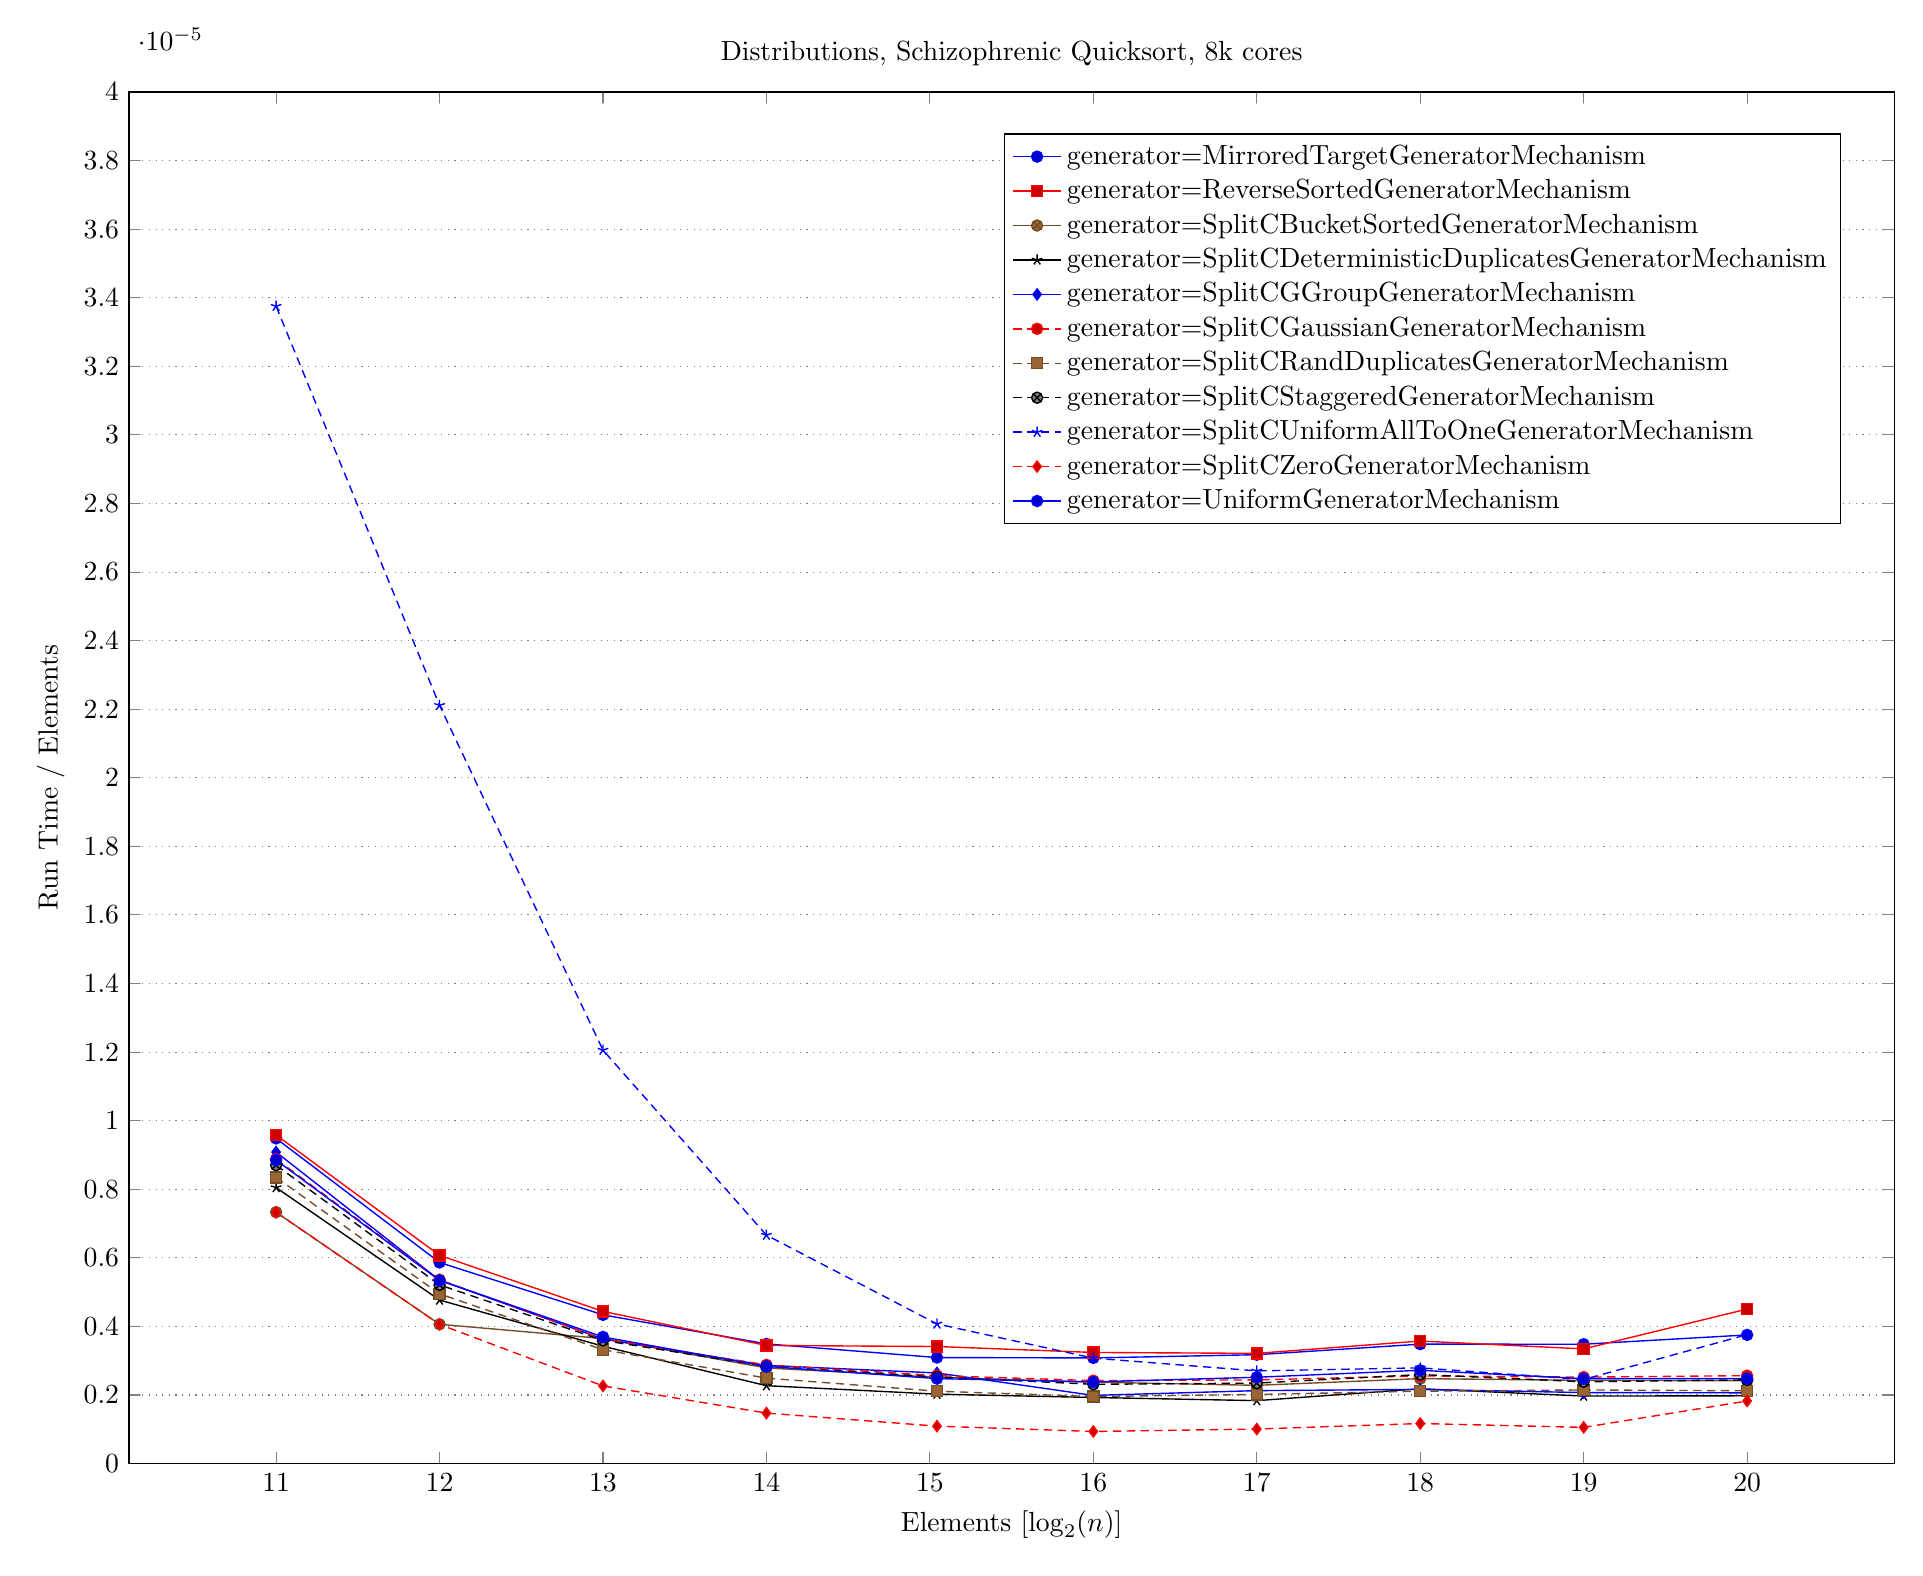
\begin{tikzpicture}
  \begin{axis}[
    title={Distributions, Schizophrenic Quicksort, 8k cores},
    xlabel={Elements [$\log_2(n)$]},
    ylabel={Run Time / Elements},
    xmajorgrids=false,
    xtick={0,...,20},
    ymin=0,   
    ymax=4e-5,
    ]   
	%% MULTIPLOT(generator) SELECT  LOG(2,`n-p`) AS x, MEDIAN(`wall-time`)/`n-p` as y, MULTIPLOT
	%% FROM ResultsQS
	%% WHERE p=8192  AND algo="SchizoQSDistTwoDistSorterMechanism" AND x>=11
	%% GROUP BY MULTIPLOT, x  ORDER BY MULTIPLOT, x
 \addplot coordinates { (11.0,9.48218e-06) (12.0,5.86426e-06) (13.0,4.33698e-06) (14.0,3.48984e-06) (15.0434,3.09146e-06) (16.0,3.08063e-06) (17.0,3.17468e-06) (18.0,3.48209e-06) (19.0,3.48055e-06) (20.0,3.75147e-06) };
 \addlegendentry{generator=MirroredTargetGeneratorMechanism};
 \addplot coordinates { (11.0,9.58228e-06) (12.0,6.07239e-06) (13.0,4.43805e-06) (14.0,3.44379e-06) (15.0434,3.41344e-06) (16.0,3.2402e-06) (17.0,3.21365e-06) (18.0,3.57321e-06) (19.0,3.34367e-06) (20.0,4.50538e-06) };
 \addlegendentry{generator=ReverseSortedGeneratorMechanism};
 \addplot coordinates { (11.0,7.33179e-06) (12.0,4.06165e-06) (13.0,3.64679e-06) (14.0,2.78836e-06) (15.0434,2.51735e-06) (16.0,2.37444e-06) (17.0,2.2815e-06) (18.0,2.47702e-06) (19.0,2.42677e-06) (20.0,2.41475e-06) };
 \addlegendentry{generator=SplitCBucketSortedGeneratorMechanism};
 \addplot coordinates { (11.0,8.0481e-06) (12.0,4.76843e-06) (13.0,3.42145e-06) (14.0,2.271e-06) (15.0434,2.02388e-06) (16.0,1.92707e-06) (17.0,1.83484e-06) (18.0,2.18202e-06) (19.0,1.96847e-06) (20.0,1.97652e-06) };
 \addlegendentry{generator=SplitCDeterministicDuplicatesGeneratorMechanism};
 \addplot coordinates { (11.0,9.08374e-06) (12.0,5.34802e-06) (13.0,3.63306e-06) (14.0,2.86215e-06) (15.0434,2.64219e-06) (16.0,1.98754e-06) (17.0,2.12657e-06) (18.0,2.16239e-06) (19.0,2.07046e-06) (20.0,2.06249e-06) };
 \addlegendentry{generator=SplitCGGroupGeneratorMechanism};
 \addplot coordinates { (11.0,8.87915e-06) (12.0,5.36096e-06) (13.0,3.63196e-06) (14.0,2.87866e-06) (15.0434,2.56395e-06) (16.0,2.41938e-06) (17.0,2.43973e-06) (18.0,2.55678e-06) (19.0,2.52129e-06) (20.0,2.56442e-06) };
 \addlegendentry{generator=SplitCGaussianGeneratorMechanism};
 \addplot coordinates { (11.0,8.34497e-06) (12.0,4.94812e-06) (13.0,3.32056e-06) (14.0,2.49176e-06) (15.0434,2.11031e-06) (16.0,1.95439e-06) (17.0,2.0155e-06) (18.0,2.10902e-06) (19.0,2.14652e-06) (20.0,2.12246e-06) };
 \addlegendentry{generator=SplitCRandDuplicatesGeneratorMechanism};
 \addplot coordinates { (11.0,8.70166e-06) (12.0,5.21094e-06) (13.0,3.59119e-06) (14.0,2.83655e-06) (15.0434,2.52517e-06) (16.0,2.31139e-06) (17.0,2.34546e-06) (18.0,2.59705e-06) (19.0,2.38569e-06) (20.0,2.44169e-06) };
 \addlegendentry{generator=SplitCStaggeredGeneratorMechanism};
 \addplot coordinates { (11.0,3.37529e-05) (12.0,2.21135e-05) (13.0,1.2058e-05) (14.0,6.66208e-06) (15.0434,4.07286e-06) (16.0,3.07427e-06) (17.0,2.70258e-06) (18.0,2.79093e-06) (19.0,2.45176e-06) (20.0,3.76034e-06) };
 \addlegendentry{generator=SplitCUniformAllToOneGeneratorMechanism};
 \addplot coordinates { (11.0,7.32764e-06) (12.0,4.05896e-06) (13.0,2.26343e-06) (14.0,1.47211e-06) (15.0434,1.09105e-06) (16.0,9.35577e-07) (17.0,1.00692e-06) (18.0,1.1678e-06) (19.0,1.05548e-06) (20.0,1.82489e-06) };
 \addlegendentry{generator=SplitCZeroGeneratorMechanism};
 \addplot coordinates { (11.0,8.84961e-06) (12.0,5.34277e-06) (13.0,3.69324e-06) (14.0,2.83298e-06) (15.0434,2.47758e-06) (16.0,2.38049e-06) (17.0,2.51684e-06) (18.0,2.71963e-06) (19.0,2.47575e-06) (20.0,2.47925e-06) };
 \addlegendentry{generator=UniformGeneratorMechanism};

  \end{axis}
\end{tikzpicture}
\newpage

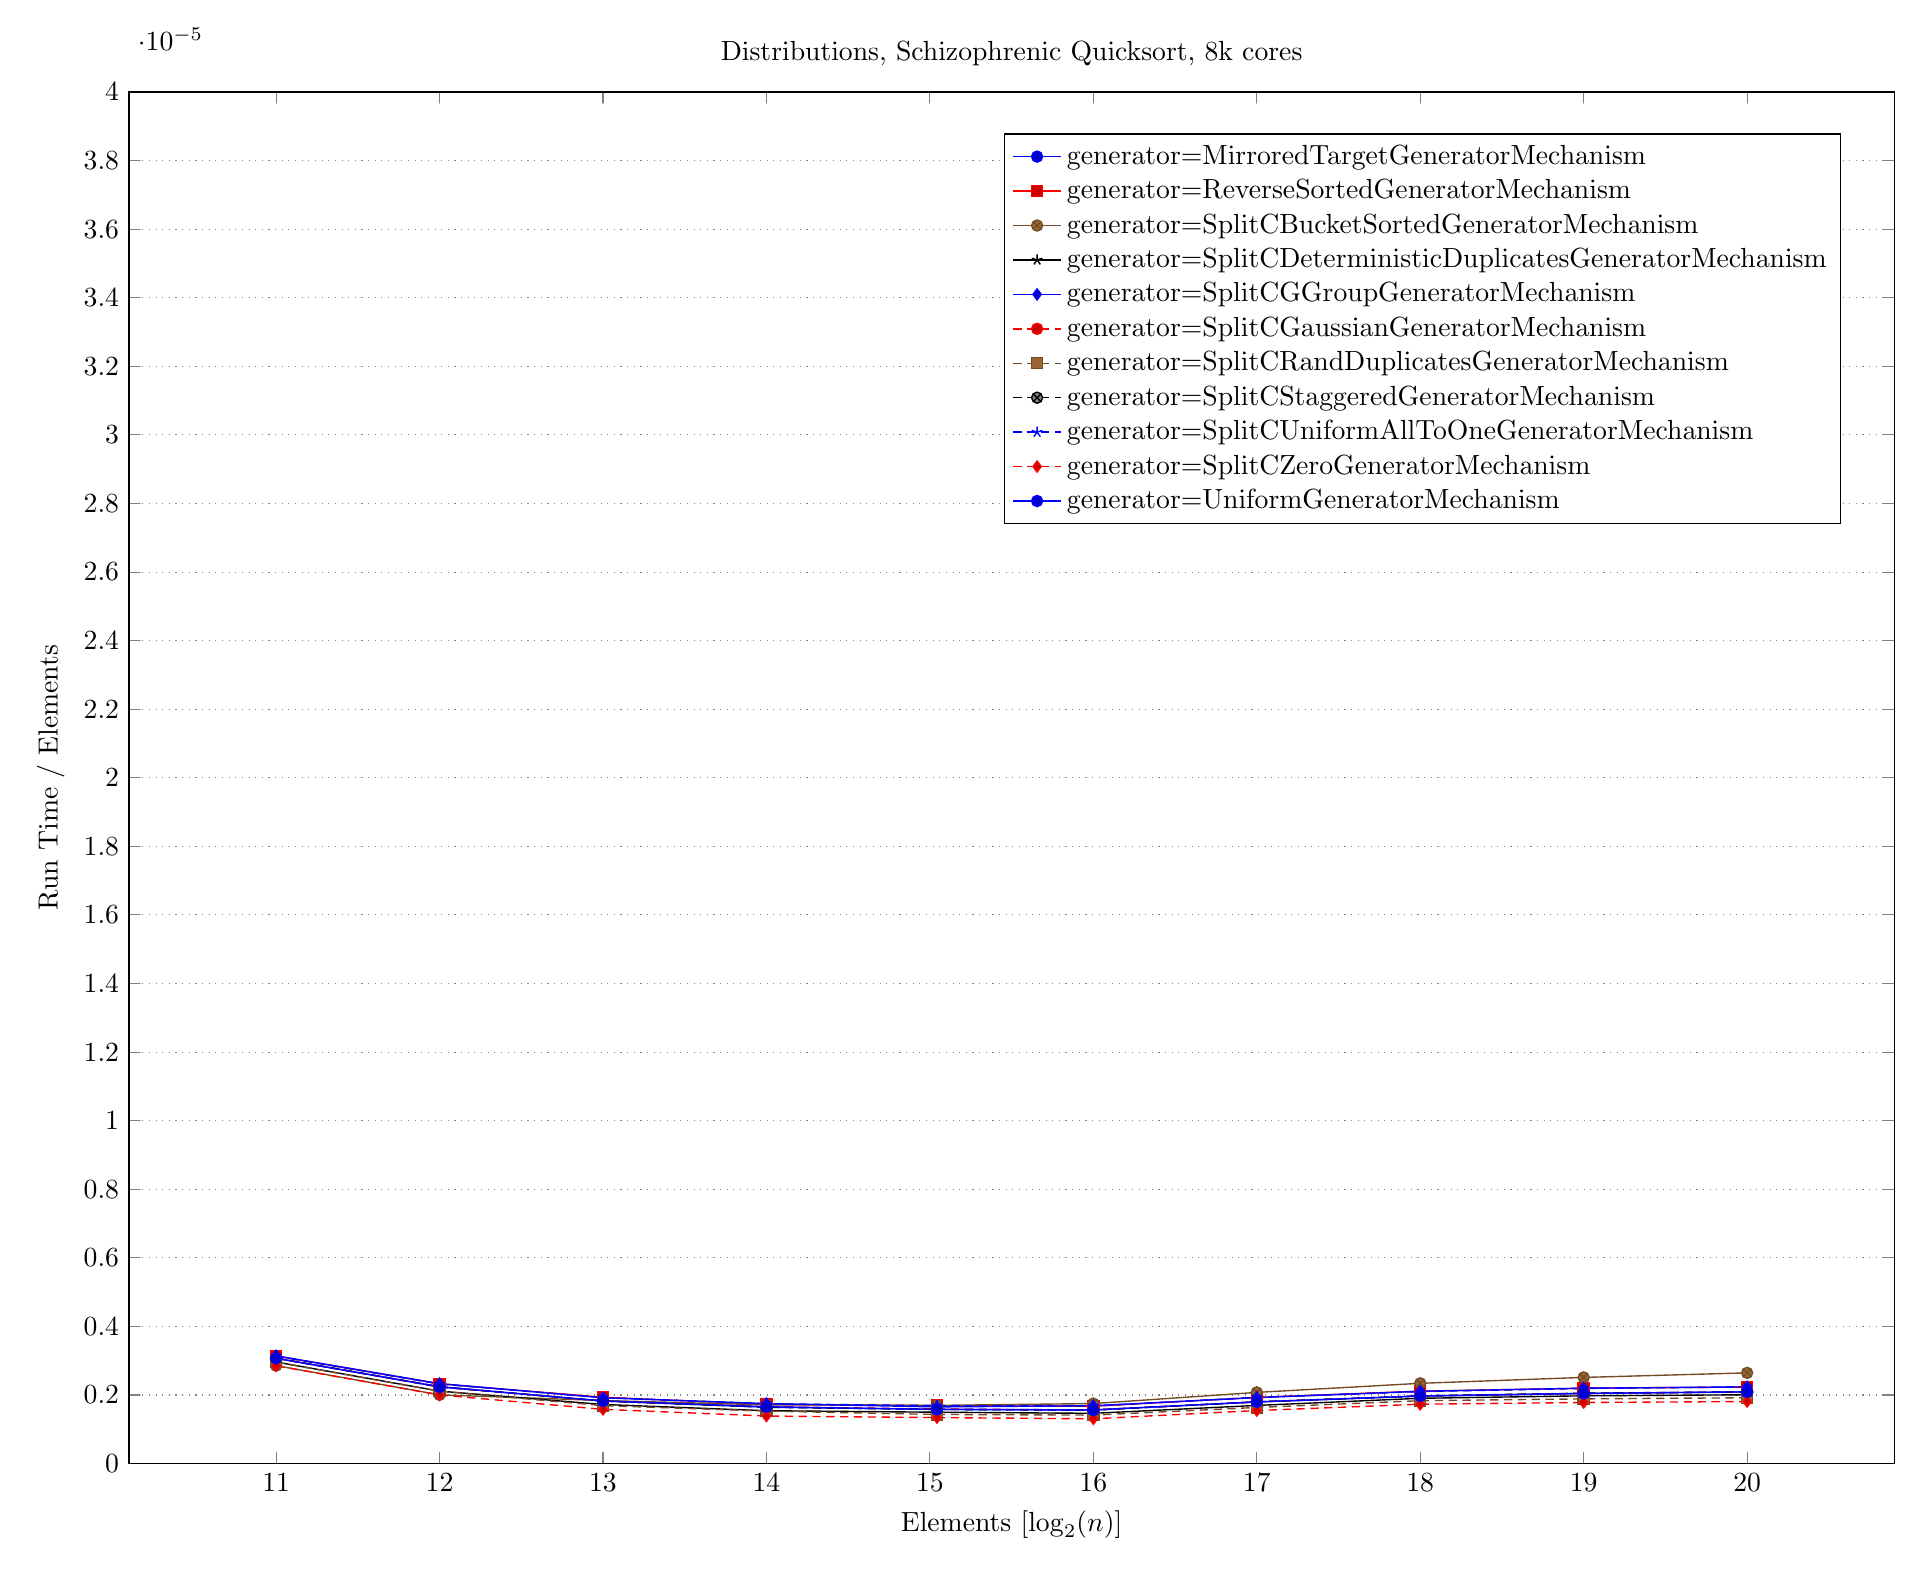
\begin{tikzpicture}
  \begin{axis}[
    title={Distributions, Schizophrenic Quicksort, 8k cores},
    xlabel={Elements [$\log_2(n)$]},
    ylabel={Run Time / Elements},
    xmajorgrids=false,
    xtick={0,...,20},
    ymin=0,   
    ymax=4e-5,
    ]   
	%% MULTIPLOT(generator) SELECT  LOG(2,`n-p`) AS x, MEDIAN(`wall-time`)/`n-p` as y, MULTIPLOT
	%% FROM ResultsQS
	%% WHERE p=8192  AND algo="LightSplitParQsortDistTwoDistSorterMechanism<LightSplitBinTreeKMedianSelect,KNeighborhoodPivotSelectorMechanism>" AND x>=11
	%% GROUP BY MULTIPLOT, x  ORDER BY MULTIPLOT, x
 \addplot coordinates { (11.0,3.07031e-06) (12.0,2.24121e-06) (13.0,1.82397e-06) (14.0,1.64462e-06) (15.0434,1.58246e-06) (16.0,1.56477e-06) (17.0,1.79682e-06) (18.0,1.96509e-06) (19.0,2.044e-06) (20.0,2.09091e-06) };
 \addlegendentry{generator=MirroredTargetGeneratorMechanism};
 \addplot coordinates { (11.0,3.13281e-06) (12.0,2.32263e-06) (13.0,1.93451e-06) (14.0,1.73047e-06) (15.0434,1.68797e-06) (16.0,1.67177e-06) (17.0,1.92995e-06) (18.0,2.11134e-06) (19.0,2.19795e-06) (20.0,2.23122e-06) };
 \addlegendentry{generator=ReverseSortedGeneratorMechanism};
 \addplot coordinates { (11.0,2.85547e-06) (12.0,2.00415e-06) (13.0,1.83844e-06) (14.0,1.71204e-06) (15.0434,1.69696e-06) (16.0,1.74905e-06) (17.0,2.07511e-06) (18.0,2.34019e-06) (19.0,2.51232e-06) (20.0,2.64485e-06) };
 \addlegendentry{generator=SplitCBucketSortedGeneratorMechanism};
 \addplot coordinates { (11.0,2.96191e-06) (12.0,2.11255e-06) (13.0,1.7229e-06) (14.0,1.54117e-06) (15.0434,1.49728e-06) (16.0,1.46487e-06) (17.0,1.69521e-06) (18.0,1.90367e-06) (19.0,1.97515e-06) (20.0,2.00606e-06) };
 \addlegendentry{generator=SplitCDeterministicDuplicatesGeneratorMechanism};
 \addplot coordinates { (11.0,3.14258e-06) (12.0,2.33215e-06) (13.0,1.91693e-06) (14.0,1.74899e-06) (15.0434,1.65201e-06) (16.0,1.68629e-06) (17.0,1.92235e-06) (18.0,2.10725e-06) (19.0,2.19773e-06) (20.0,2.23546e-06) };
 \addlegendentry{generator=SplitCGGroupGeneratorMechanism};
 \addplot coordinates { (11.0,3.07349e-06) (12.0,2.22925e-06) (13.0,1.82184e-06) (14.0,1.65671e-06) (15.0434,1.59032e-06) (16.0,1.56336e-06) (17.0,1.8001e-06) (18.0,1.97028e-06) (19.0,2.04377e-06) (20.0,2.0838e-06) };
 \addlegendentry{generator=SplitCGaussianGeneratorMechanism};
 \addplot coordinates { (11.0,2.95679e-06) (12.0,2.11011e-06) (13.0,1.68927e-06) (14.0,1.53079e-06) (15.0434,1.43177e-06) (16.0,1.41315e-06) (17.0,1.63572e-06) (18.0,1.83325e-06) (19.0,1.8865e-06) (20.0,1.91889e-06) };
 \addlegendentry{generator=SplitCRandDuplicatesGeneratorMechanism};
 \addplot coordinates { (11.0,3.07153e-06) (12.0,2.24121e-06) (13.0,1.82489e-06) (14.0,1.64127e-06) (15.0434,1.57891e-06) (16.0,1.5564e-06) (17.0,1.79869e-06) (18.0,1.97389e-06) (19.0,2.05319e-06) (20.0,2.08972e-06) };
 \addlegendentry{generator=SplitCStaggeredGeneratorMechanism};
 \addplot coordinates { (11.0,3.13257e-06) (12.0,2.32007e-06) (13.0,1.92358e-06) (14.0,1.74438e-06) (15.0434,1.68897e-06) (16.0,1.67705e-06) (17.0,1.93087e-06) (18.0,2.09803e-06) (19.0,2.1902e-06) (20.0,2.23466e-06) };
 \addlegendentry{generator=SplitCUniformAllToOneGeneratorMechanism};
 \addplot coordinates { (11.0,2.85254e-06) (12.0,2.00146e-06) (13.0,1.58105e-06) (14.0,1.38687e-06) (15.0434,1.34001e-06) (16.0,1.30568e-06) (17.0,1.54655e-06) (18.0,1.73116e-06) (19.0,1.78137e-06) (20.0,1.80844e-06) };
 \addlegendentry{generator=SplitCZeroGeneratorMechanism};
 \addplot coordinates { (11.0,3.0708e-06) (12.0,2.23474e-06) (13.0,1.82654e-06) (14.0,1.6568e-06) (15.0434,1.57771e-06) (16.0,1.56219e-06) (17.0,1.79824e-06) (18.0,1.97251e-06) (19.0,2.04606e-06) (20.0,2.09116e-06) };
 \addlegendentry{generator=UniformGeneratorMechanism};

  \end{axis}
\end{tikzpicture}
\newpage

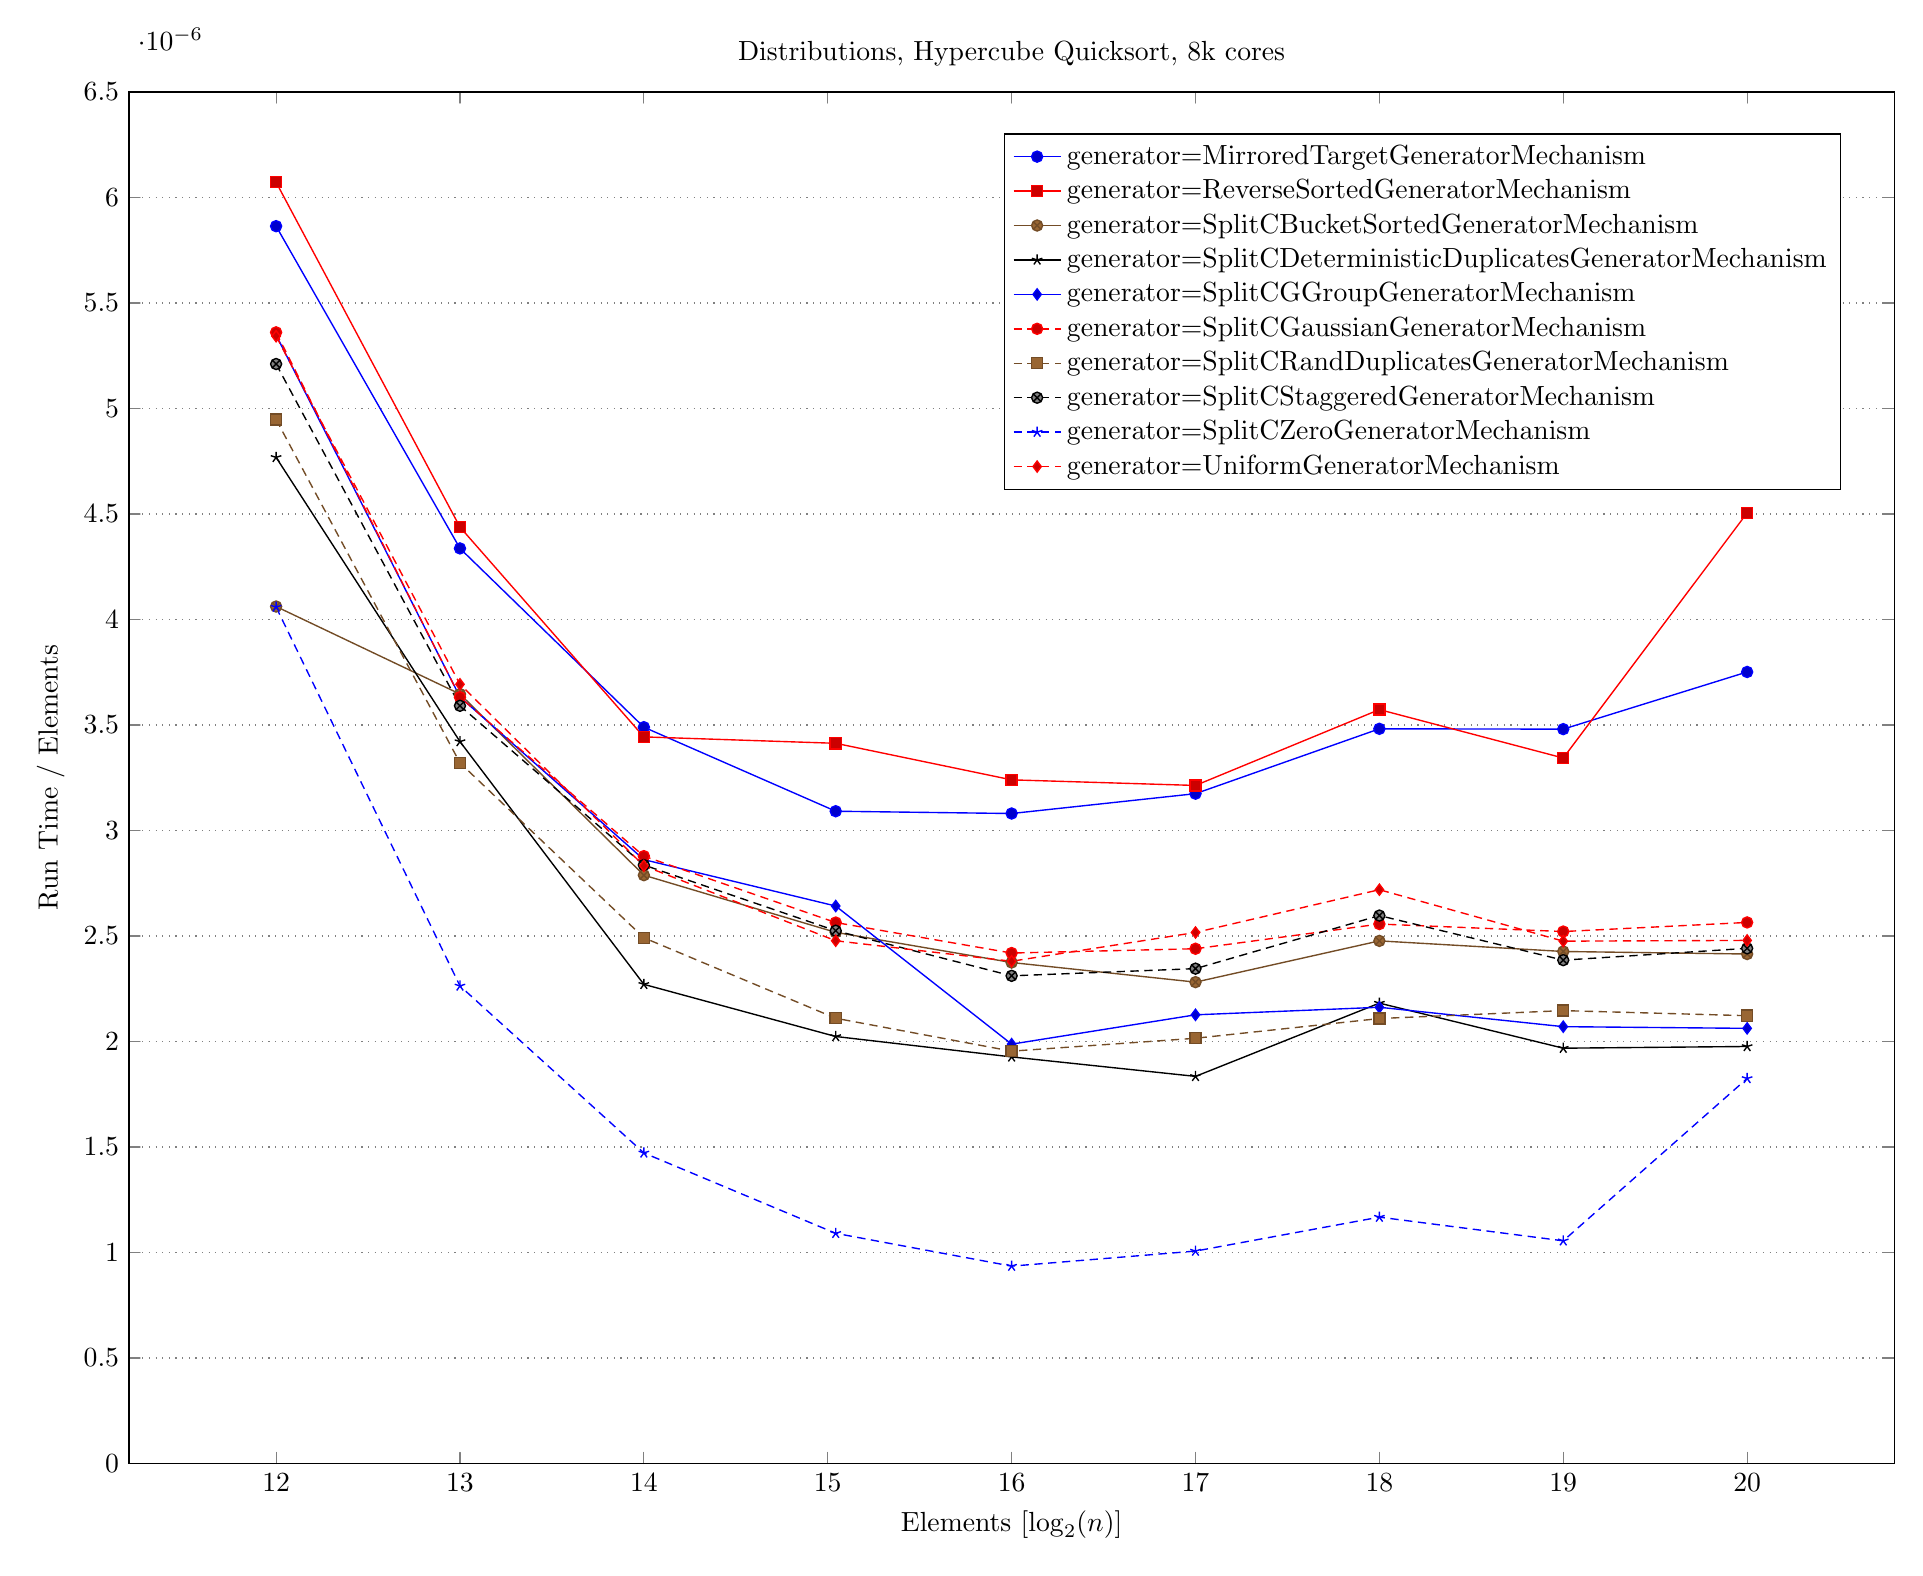
\begin{tikzpicture}
  \begin{axis}[
    title={Distributions, Hypercube Quicksort, 8k cores},
    xlabel={Elements [$\log_2(n)$]},
    ylabel={Run Time / Elements},
    xmajorgrids=false,
    xtick={0,...,20},
    ymin=0,
    ymax=6.5e-6,
    ]   
	%% MULTIPLOT(generator) SELECT  LOG(2,`n-p`) AS x, MEDIAN(`wall-time`)/`n-p` as y, MULTIPLOT
	%% FROM ResultsQS
	%% WHERE p=8192  AND algo="SchizoQSDistTwoDistSorterMechanism" AND NOT generator="SplitCUniformAllToOneGeneratorMechanism" AND x>=12
	%% GROUP BY MULTIPLOT, x  ORDER BY MULTIPLOT, x
 \addplot coordinates { (12.0,5.86426e-06) (13.0,4.33698e-06) (14.0,3.48984e-06) (15.0434,3.09146e-06) (16.0,3.08063e-06) (17.0,3.17468e-06) (18.0,3.48209e-06) (19.0,3.48055e-06) (20.0,3.75147e-06) };
 \addlegendentry{generator=MirroredTargetGeneratorMechanism};
 \addplot coordinates { (12.0,6.07239e-06) (13.0,4.43805e-06) (14.0,3.44379e-06) (15.0434,3.41344e-06) (16.0,3.2402e-06) (17.0,3.21365e-06) (18.0,3.57321e-06) (19.0,3.34367e-06) (20.0,4.50538e-06) };
 \addlegendentry{generator=ReverseSortedGeneratorMechanism};
 \addplot coordinates { (12.0,4.06165e-06) (13.0,3.64679e-06) (14.0,2.78836e-06) (15.0434,2.51735e-06) (16.0,2.37444e-06) (17.0,2.2815e-06) (18.0,2.47702e-06) (19.0,2.42677e-06) (20.0,2.41475e-06) };
 \addlegendentry{generator=SplitCBucketSortedGeneratorMechanism};
 \addplot coordinates { (12.0,4.76843e-06) (13.0,3.42145e-06) (14.0,2.271e-06) (15.0434,2.02388e-06) (16.0,1.92707e-06) (17.0,1.83484e-06) (18.0,2.18202e-06) (19.0,1.96847e-06) (20.0,1.97652e-06) };
 \addlegendentry{generator=SplitCDeterministicDuplicatesGeneratorMechanism};
 \addplot coordinates { (12.0,5.34802e-06) (13.0,3.63306e-06) (14.0,2.86215e-06) (15.0434,2.64219e-06) (16.0,1.98754e-06) (17.0,2.12657e-06) (18.0,2.16239e-06) (19.0,2.07046e-06) (20.0,2.06249e-06) };
 \addlegendentry{generator=SplitCGGroupGeneratorMechanism};
 \addplot coordinates { (12.0,5.36096e-06) (13.0,3.63196e-06) (14.0,2.87866e-06) (15.0434,2.56395e-06) (16.0,2.41938e-06) (17.0,2.43973e-06) (18.0,2.55678e-06) (19.0,2.52129e-06) (20.0,2.56442e-06) };
 \addlegendentry{generator=SplitCGaussianGeneratorMechanism};
 \addplot coordinates { (12.0,4.94812e-06) (13.0,3.32056e-06) (14.0,2.49176e-06) (15.0434,2.11031e-06) (16.0,1.95439e-06) (17.0,2.0155e-06) (18.0,2.10902e-06) (19.0,2.14652e-06) (20.0,2.12246e-06) };
 \addlegendentry{generator=SplitCRandDuplicatesGeneratorMechanism};
 \addplot coordinates { (12.0,5.21094e-06) (13.0,3.59119e-06) (14.0,2.83655e-06) (15.0434,2.52517e-06) (16.0,2.31139e-06) (17.0,2.34546e-06) (18.0,2.59705e-06) (19.0,2.38569e-06) (20.0,2.44169e-06) };
 \addlegendentry{generator=SplitCStaggeredGeneratorMechanism};
 \addplot coordinates { (12.0,4.05896e-06) (13.0,2.26343e-06) (14.0,1.47211e-06) (15.0434,1.09105e-06) (16.0,9.35577e-07) (17.0,1.00692e-06) (18.0,1.1678e-06) (19.0,1.05548e-06) (20.0,1.82489e-06) };
 \addlegendentry{generator=SplitCZeroGeneratorMechanism};
 \addplot coordinates { (12.0,5.34277e-06) (13.0,3.69324e-06) (14.0,2.83298e-06) (15.0434,2.47758e-06) (16.0,2.38049e-06) (17.0,2.51684e-06) (18.0,2.71963e-06) (19.0,2.47575e-06) (20.0,2.47925e-06) };
 \addlegendentry{generator=UniformGeneratorMechanism};

  \end{axis}
\end{tikzpicture}
\newpage

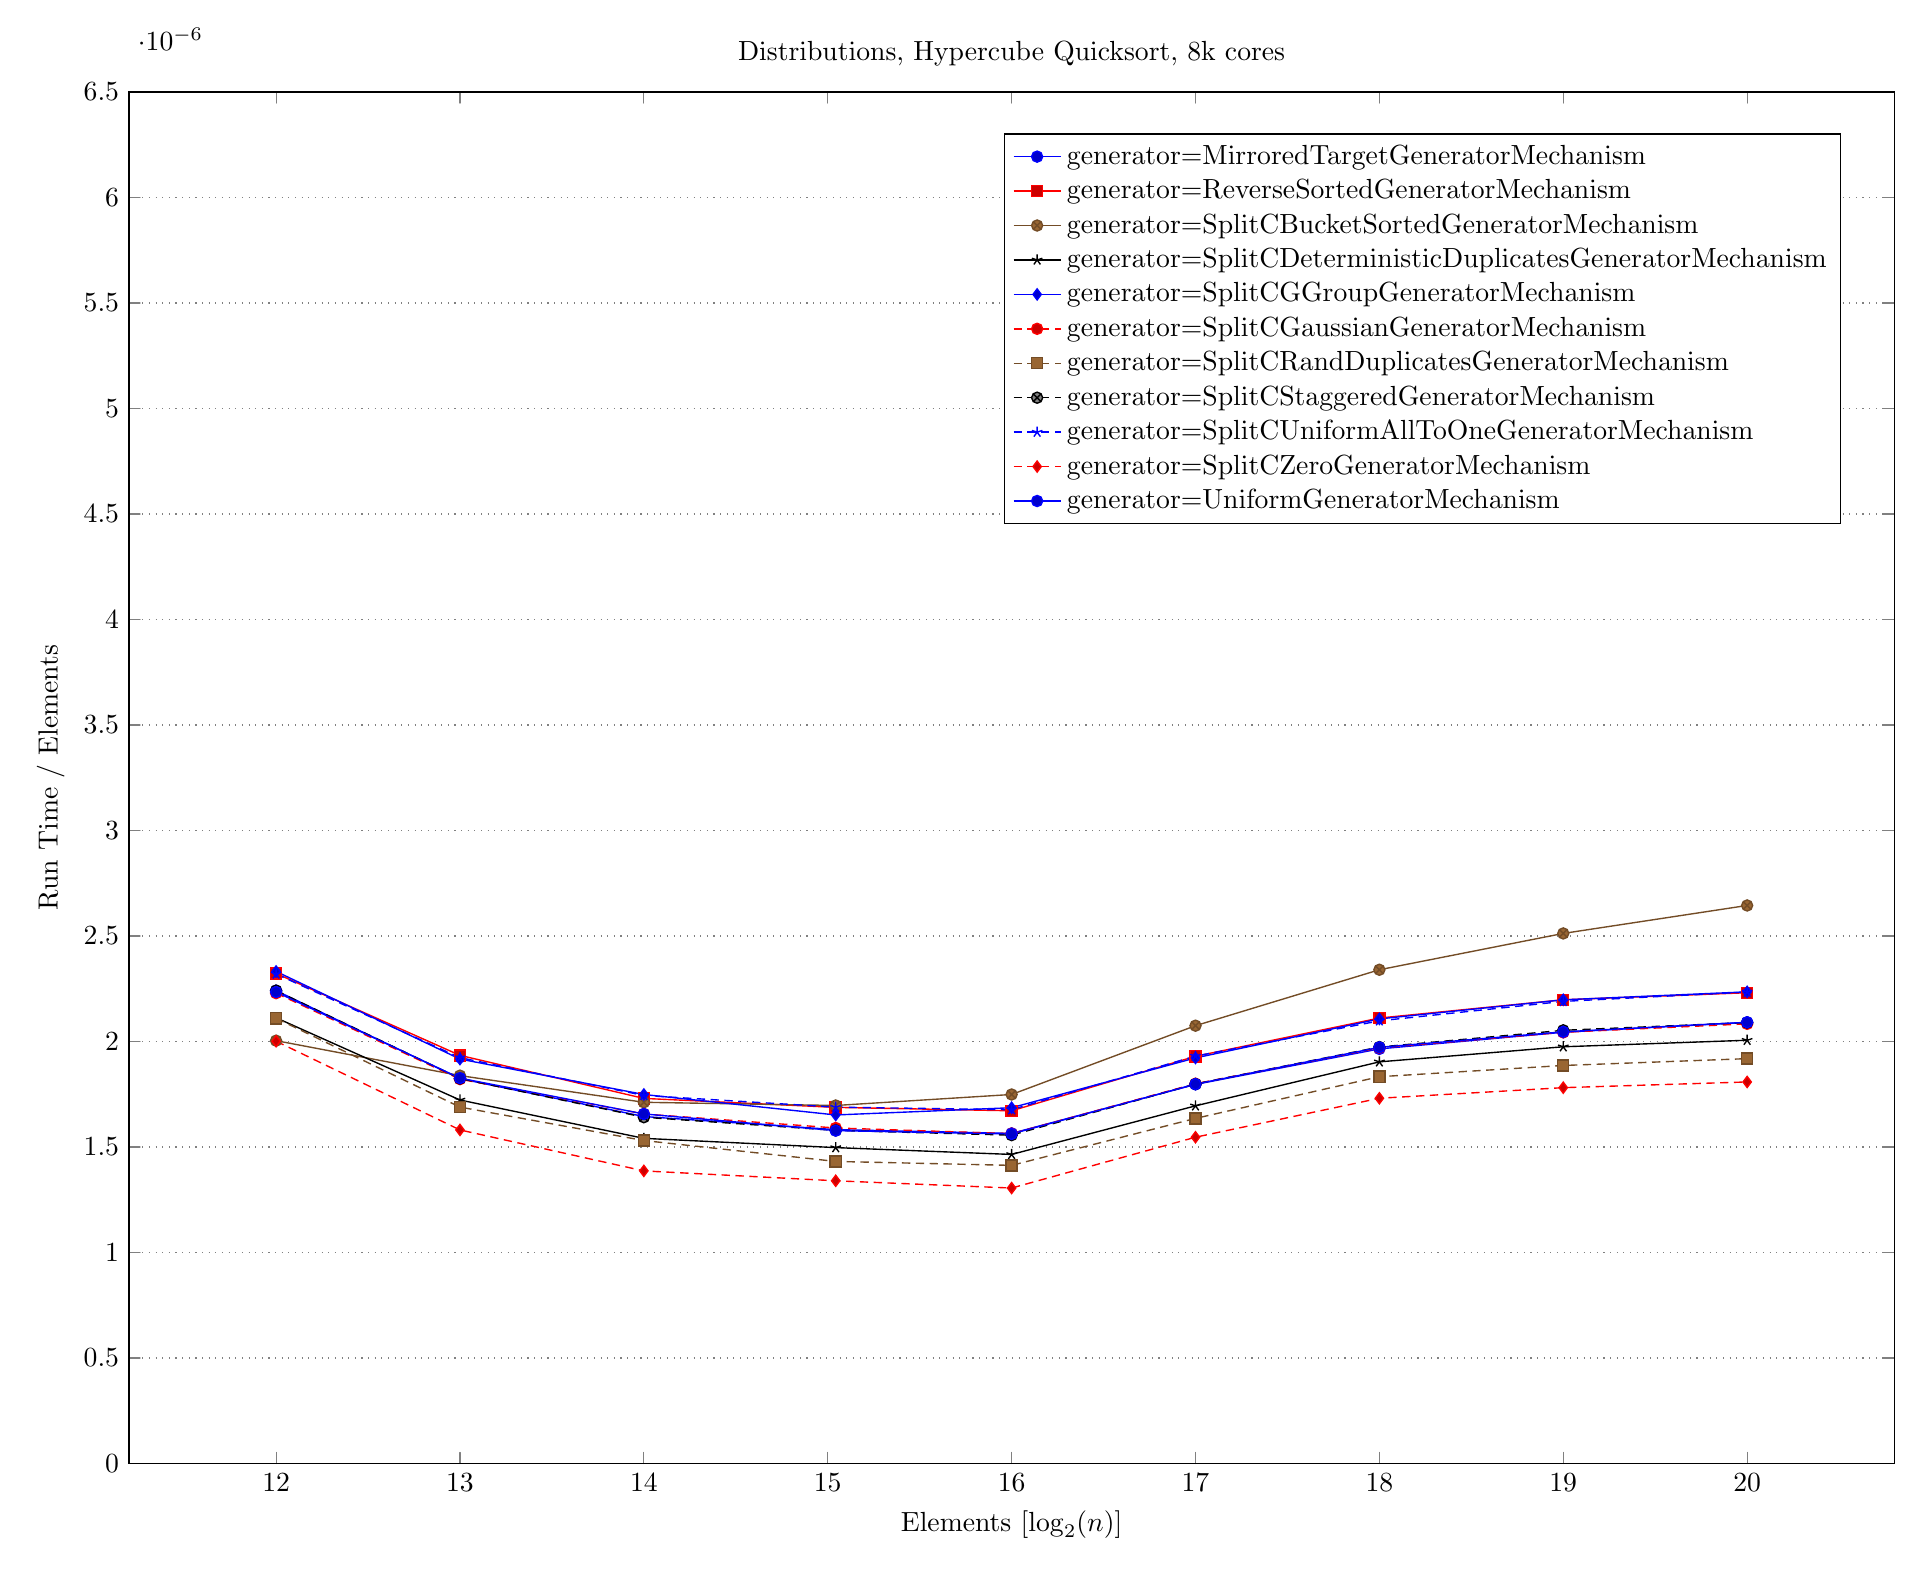
\begin{tikzpicture}
  \begin{axis}[
    title={Distributions, Hypercube Quicksort, 8k cores},
    xlabel={Elements [$\log_2(n)$]},
    ylabel={Run Time / Elements},
    xmajorgrids=false,
    xtick={0,...,20},
    ymin=0,
    ymax=6.5e-6,
    ]   
	%% MULTIPLOT(generator) SELECT  LOG(2,`n-p`) AS x, MEDIAN(`wall-time`)/`n-p` as y, MULTIPLOT
	%% FROM ResultsQS
	%% WHERE p=8192  AND algo="LightSplitParQsortDistTwoDistSorterMechanism<LightSplitBinTreeKMedianSelect,KNeighborhoodPivotSelectorMechanism>" AND x>=12
	%% GROUP BY MULTIPLOT, x  ORDER BY MULTIPLOT, x
 \addplot coordinates { (12.0,2.24121e-06) (13.0,1.82397e-06) (14.0,1.64462e-06) (15.0434,1.58246e-06) (16.0,1.56477e-06) (17.0,1.79682e-06) (18.0,1.96509e-06) (19.0,2.044e-06) (20.0,2.09091e-06) };
 \addlegendentry{generator=MirroredTargetGeneratorMechanism};
 \addplot coordinates { (12.0,2.32263e-06) (13.0,1.93451e-06) (14.0,1.73047e-06) (15.0434,1.68797e-06) (16.0,1.67177e-06) (17.0,1.92995e-06) (18.0,2.11134e-06) (19.0,2.19795e-06) (20.0,2.23122e-06) };
 \addlegendentry{generator=ReverseSortedGeneratorMechanism};
 \addplot coordinates { (12.0,2.00415e-06) (13.0,1.83844e-06) (14.0,1.71204e-06) (15.0434,1.69696e-06) (16.0,1.74905e-06) (17.0,2.07511e-06) (18.0,2.34019e-06) (19.0,2.51232e-06) (20.0,2.64485e-06) };
 \addlegendentry{generator=SplitCBucketSortedGeneratorMechanism};
 \addplot coordinates { (12.0,2.11255e-06) (13.0,1.7229e-06) (14.0,1.54117e-06) (15.0434,1.49728e-06) (16.0,1.46487e-06) (17.0,1.69521e-06) (18.0,1.90367e-06) (19.0,1.97515e-06) (20.0,2.00606e-06) };
 \addlegendentry{generator=SplitCDeterministicDuplicatesGeneratorMechanism};
 \addplot coordinates { (12.0,2.33215e-06) (13.0,1.91693e-06) (14.0,1.74899e-06) (15.0434,1.65201e-06) (16.0,1.68629e-06) (17.0,1.92235e-06) (18.0,2.10725e-06) (19.0,2.19773e-06) (20.0,2.23546e-06) };
 \addlegendentry{generator=SplitCGGroupGeneratorMechanism};
 \addplot coordinates { (12.0,2.22925e-06) (13.0,1.82184e-06) (14.0,1.65671e-06) (15.0434,1.59032e-06) (16.0,1.56336e-06) (17.0,1.8001e-06) (18.0,1.97028e-06) (19.0,2.04377e-06) (20.0,2.0838e-06) };
 \addlegendentry{generator=SplitCGaussianGeneratorMechanism};
 \addplot coordinates { (12.0,2.11011e-06) (13.0,1.68927e-06) (14.0,1.53079e-06) (15.0434,1.43177e-06) (16.0,1.41315e-06) (17.0,1.63572e-06) (18.0,1.83325e-06) (19.0,1.8865e-06) (20.0,1.91889e-06) };
 \addlegendentry{generator=SplitCRandDuplicatesGeneratorMechanism};
 \addplot coordinates { (12.0,2.24121e-06) (13.0,1.82489e-06) (14.0,1.64127e-06) (15.0434,1.57891e-06) (16.0,1.5564e-06) (17.0,1.79869e-06) (18.0,1.97389e-06) (19.0,2.05319e-06) (20.0,2.08972e-06) };
 \addlegendentry{generator=SplitCStaggeredGeneratorMechanism};
 \addplot coordinates { (12.0,2.32007e-06) (13.0,1.92358e-06) (14.0,1.74438e-06) (15.0434,1.68897e-06) (16.0,1.67705e-06) (17.0,1.93087e-06) (18.0,2.09803e-06) (19.0,2.1902e-06) (20.0,2.23466e-06) };
 \addlegendentry{generator=SplitCUniformAllToOneGeneratorMechanism};
 \addplot coordinates { (12.0,2.00146e-06) (13.0,1.58105e-06) (14.0,1.38687e-06) (15.0434,1.34001e-06) (16.0,1.30568e-06) (17.0,1.54655e-06) (18.0,1.73116e-06) (19.0,1.78137e-06) (20.0,1.80844e-06) };
 \addlegendentry{generator=SplitCZeroGeneratorMechanism};
 \addplot coordinates { (12.0,2.23474e-06) (13.0,1.82654e-06) (14.0,1.6568e-06) (15.0434,1.57771e-06) (16.0,1.56219e-06) (17.0,1.79824e-06) (18.0,1.97251e-06) (19.0,2.04606e-06) (20.0,2.09116e-06) };
 \addlegendentry{generator=UniformGeneratorMechanism};

  \end{axis}
\end{tikzpicture}
\newpage

\end{center}

\end{document}

%%%%%%%%%%%%%%%%%%%%%%%%%%%%%%%%%%%%%%%%%%%%%%%%%%%%%%%%%%%%%%%%%%%%%%%%%%%%%%%%
